% !TeX root = ../../../main.tex
\section{Results}

Table~\ref{tbl:demographics} summarizes the demographics of the 64 patients included in this study. All patients received standard immunosuppressive therapies regardless of study participation. No significant differences were observed between participants' age, sex, BMI, donor types, whether zero-hour biopsies were performed, and the number of indication biopsies except for whether a zero-hour biopsy was performed on a graft and whether it came from a living donor ($p$~=~0.34, Spearman's rank correlation coefficient $\rho$~=~0.27). For racial/ethnic groups, significant correlations were observed between whether participants were White and the number of indication biopsies performed ($p$~=~0.049, $\rho$~=~-0.25) and whether grafts came from a living donor ($p$~=~0.0018, $\rho$~=~0.39), whether participants were Black and whether donors were living ($p$~=~0.0023, $\rho$~=~-0.39), whether participants were Hispanic/Latinx and underwent zero-hour biopsies ($p$~=~0.043, $\rho$~=~0.26), and between the number of indication biopsies performed whether a participant was Asian ($p$~=~0.024, $\rho$~=~0.29). Regarding the reasons for study withdrawals, excluding demographic groups with 5 or fewer participants and study withdrawal reasons unrelated to pathology, noncompliance, or consent, the only significant difference observed was between the number of indication biopsies and whether a participant ended study participation due to a clinical diagnosis of graft rejection ($p$~=~0.0030, $\rho$~=~0.38). The singular death occurred in a patient who did not undergo any indication biopsies during their study participation, and was caused by an unrelated comorbidity.

% Table of patient demographics
% !TeX root = ../../../main.tex

\begin{table}[tbp]
    \centering
    \caption{Demographics of Patients Included in This Study}
    \begin{tabular}{lrr}
        \toprule
        Participants & 
        \multicolumn{2}{c}{64~Total*}\\\midrule
        Male / Female & \multicolumn{2}{c}{35 / 29} \\
        BMI at Transplantation (\unit{\kilo\gram\per\meter\squared}) & \multicolumn{2}{c}{27.6 $\pm$ 5.3} \\
        Age at Transplantation & & \\
        \hspace{2em}\textless 35 years & 10 & (15.6 \%)\\
        \hspace{2em}35--50 years & 17 & (26.6 \%)\\
        \hspace{2em}51--65 years & 27 & (42.2 \%)\\
        \hspace{2em}\textgreater 65 years & 10 & (15.6 \%)\\
        Race/Ethnicity & & \\
        \hspace{2em}White & 35 & (54.7 \%)\\
        \hspace{2em}Black/African American & 22 & (34.4 \%)\\
        \hspace{2em}Hispanic/Latinx & 3 & (4.7 \%)\\
        \hspace{2em}Asian & 3 & (4.7 \%)\\
        \hspace{2em}Native American & 1 & (1.6 \%)\\
        Graft from Deceased Donor & 40 & (62.5 \%)\\
        Zero-Hour Biopsy Performed & 36 & (56.3 \%)\\
        \hspace{2em}Also Underwent Indication Biopsy & 9 & (14.1 \%)\\
        Only Underwent Indication Biopsy & 10 & (15.6 \%)\\
        Number of Indication Biopsies & & \\
        \hspace{2em}None & 45 & (70.3 \%)\\
        \hspace{2em}1 & 10 & (15.6 \%)\\
        \hspace{2em}2 & 7 & (10.9 \%)\\
        \hspace{2em}3 & 1 & (1.6 \%)\\
        \hspace{2em}4 & 1 & (1.6 \%)\\
        Reason for Study Departure & & \\
        \hspace{2em}Study Termination & 35 & (54.7 \%)\\
        \hspace{2em}Completed 3 years & 20 & (31.3 \%)\\
        \hspace{2em}Lost to Follow-up & 4 & (6.3 \%)\\
        \hspace{2em}Clinically Indicated Rejection & 3 & (4.7 \%)\\
        \hspace{2em}Death & 1 & (1.6 \%)\\
        \hspace{2em}Pregnancy & 1 & (1.6 \%)\\
        \bottomrule
    \end{tabular}
    \par\vspace{0.5em}
    \noindent*: Values are mean $\pm$ standard deviation or as the number of patients unless shown otherwise.
    \label{tbl:demographics}
\end{table}

Fig.~\ref{fig:ptTime} depicts the timepoints at which VisR imaging was performed for each patient in the study, ordered by the duration between transplant and final imaging date. Imaging dates that are not associated with clinically indicated biopsies are marked as hollow circles, whereas those that are associated with biopsies are marked as filled diamonds. The median number of imaging dates per patient was 3 (interquartile range of 2--6), and the median duration between transplant and final imaging date was 486 days (interquartile range of 268--852 days). The number of imaging dates per patient was significantly correlated with whether participants were male ($p$~=~0.0070, $\rho$~=~0.34), whether the graft came from a living donor ($p$~=~0.050, $\rho$~=~0.25), whether a zero-hour biopsy was performed ($p$~=~0.0062, $\rho$~=~0.35), and the number of indication biopsies performed ($p$~=~0.046, $\rho$~=~0.26). The total duration between transplant and final imaging date was significantly correlated with whether participants were male ($p$~=~0.047, $\rho$~=~0.26) and whether a zero-hour biopsy was performed ($p$~=~0.012, $\rho$~=~0.32). No significant differences were found when the number of imaging dates per patient or the duration between transplant and final imaging dates were compared to participants' ages, races/ethnicities, or reasons for study withdrawal pertaining to pathology, noncompliance, or consent.

% Timeline of each patient's participation duration + imaging dates
%
% Things that I may or may not want to add:
% - second subfigure that shows the same timeline relative to the final biopsy
% - indicate biopsy findings (e.g. i, IFTA, glomerulopathy)
\begin{figure}[tb]
    \centering
    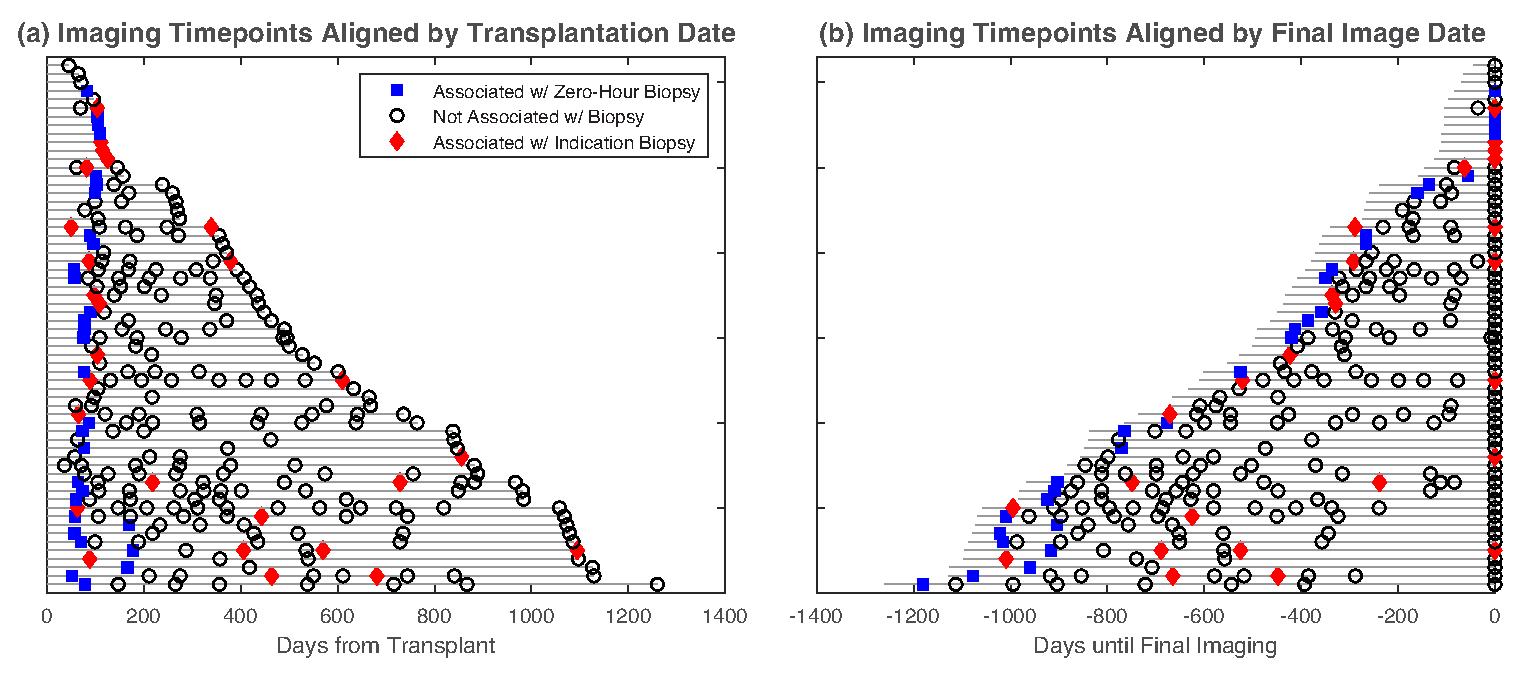
\includegraphics[width=0.9\textwidth]{parts/transplant/figs/ptDuration.eps}
    \caption{Timepoints of VisR imaging for each patient in the study, ordered by duration between transplant and final imaging date. Hollow circles, red diamonds, and blue squares indicate relationships between imaging dates and biopsies as indicated in the legend. (a) denotes time since transplant, whereas (b) denotes time until final imaging.}
    \label{fig:ptTime}
\end{figure}

67 biopsies were performed during the course of this study. Two out of 31 indication biopsies, each of which were for different patients, and 34 of 36 zero-hour biopsies were not associated with any pathological findings. Two zero-hour biopsies and the remaining 29 indication biopsies resulted in at least one pathological finding. A summary of findings, as well as justifications for biopsies performed, are given in Table~\ref{tbl:biopsy}. While the primary endpoint for this study was rejection, other pathologies such as toxicity effects from calcineurin inhibitors (CNI) such as tacrolimus, focal and segmental glomerulosclerosis (FSGS), IFTA, immunoglobulin A (IgA) nephropathy, polyomavirus nephropathy (PVN) including BK virus infections, and thrombotic microangiopathy (TMA) were also observed.

A summary of Banff scores for each biopsy is provided in Table~\ref{tbl:banffScores}. Note that many biopsies exhibited multiple pathological findings, and thus the counts of individual findings do not sum to the total number of pathological biopsies. Some patients underwent multiple indication biopsies, and not all biopsies were associated with VisR image metrics due to timing mismatches between biopsy dates and imaging dates where appropriate ROIs could be drawn. No peritubular capillaritis (ptc) or mesangial matrix expansion (mm) greater than zero were observed in any biopsies performed in this study.

% Table of biopsy justifications and findings
% !TeX root = ../../../main.tex

\begin{table}[tbp]
    \centering
    \caption{Justifications and Findings of Biopsies by Type and Headcount}
    {\small
    \begin{tabular}{l rr rr rr}
        \toprule
        Parameter & 
        \multicolumn{2}{c}{67~Biopsies} & 
        \multicolumn{2}{c}{46~Patients} & 
        \multicolumn{2}{c}{4~Rejections*} \\\midrule
        Never Biopsied & 
        - & - & 29 & (45.3 \%) & - & - \\
        Zero-Hour Biopsies & 
        36 & (53.7 \%) & 36 & (78.3 \%) & & - \\
        Indication Biopsies & 
        31 & (46.3 \%) & 19 & (41.3 \%) & 4 & (100 \%) \\
        \hspace{2em}High Serum Creatinine Only & 
        17 & (25.4 \%) & 11 & (23.9 \%) & 3 & (75 \%) \\
        \hspace{2em}High UPCR/Proteinuria Only & 
        3 & (4.5 \%) & 2 & (4.3 \%) & - & - \\
        \hspace{2em}High Creatinine and UPCR/Proteinuria & 
        3 & (4.5 \%) & 3 & (6.5 \%) & - & - \\
        \hspace{2em}DSA Circulation & 
        2 & (3.0 \%) & 2 & (4.3 \%) & - & - \\
        \hspace{2em}Delayed Graft Function & 
        4 & (6.0 \%) & 4 & (8.7 \%) & 1 & (25 \%) \\
        \hspace{2em}Decoy Cells in Urine Cytology & 
        1 & (1.5 \%) & 1 & (2.2 \%) & - & - \\
        \hspace{2em}Perinephric Hematoma & 
        1 & (1.5 \%) & 1 & (2.2 \%) & 1 & (25 \%) \\
        \hline
        No Pathologies Noted &
        36 & (53.7 \%) & - & - & - & - \\
        \hspace{2em}Zero-Hour Biopsies & % Pt. 48's zero-hour biopsy was predominantly medulla, but pathologies were not reported. All remaining zero-hour biopsies EXCEPT Pt. 25, 29 were not pathological.
        34 & (50.7 \%) & 34 & (73.9 \%) & - & - \\
        \hspace{2em}Indication Biopsies & % first of Pt. 53's three indication biopsies and Pt. 57's sole indication biopsy were NOT associated with pathologies
        2 & (3.0 \%) & 2 & (4.3 \%) & - & - \\
        Pathologies Observed\textdagger & 
        31 & (46.3 \%) & 19 & (41.3 \%) & 4 & (100 \%) \\ % zero-hour biopsies for Pt. 25 and 29, as well as all indication biopsies except for the first of Pt. 53's three indication biopsies and Pt. 57's only biopsy, were pathological. Thus, 31 & - 2 + 2 = 31 pathological biopsies in total. Pt. 57 and 25 trade spots so that there are still 19 patients.
        \hspace{2em}Acute Kidney Injury & 
        5 & (7.5 \%) & 5 & (10.9 \%) & - & - \\ % 28, 29, 39, 46, 70
        \hspace{2em}Arteriosclerosis & 
        7 & (10.4 \%) & 6 & (13.0 \%) & 2 & (50 \%) \\ % 22, 28, 39, 53x2, 74, 77
        \hspace{2em}CNI Toxicity & 
        6 & (9.0 \%) & 5 & (10.9 \%) & 1 & (25 \%) \\ % 22, 28, 65, 70, 85x2
        \hspace{2em}Glomerulopathy, incl. FSGS & 
        8 & (11.9 \%) & 4 & (8.7 \%) & 1 & (25 \%) \\ % 29x2, 33x4, 39, 53
        \hspace{2em}IFTA & 
        8 & (11.9 \%) & 5 & (10.9 \%) & 1 & (25 \%) \\ % 38, 33x3, 39, 53x2, 74
        \hspace{2em}IgA Nephropathy & 
        2 & (3.0 \%) & 2 & (4.3 \%) & - & - \\ % 25, 53
        \hspace{2em}PVN & 
        8 & (11.9 \%) & 6 & (13.0 \%) & - & - \\ % 30x2, 32x2, 33, 37, 55, 59
        \hspace{2em}Suspicious for TCMR & 
        2 & (3.0 \%) & 2 & (4.3 \%) & - & - \\ % 33, 53
        \hspace{2em}TCMR & 
        4 & (6.0 \%) & 4 & (8.7 \%) & 4 & (100 \%) \\ %% 33, 39, 77, 85
        \hspace{2em}Thrombotic Microangiopathy & 
        3 & (4.5 \%) & 3 & (6.5 \%) & 1 & (25 \%) \\ % 29, 53, 77
        \bottomrule
    \end{tabular}
    \par\vspace{0.5em}
    \noindent{}Percentages are based on the total number of biopsies or patients, as appropriate. Patient counts for overall and indication biopsies without pathological findings are not given as   *: Rejections are defined based on re-assessments using the 2022 Banff criteria rather than determinations made over the course of clinical care. \textdagger{}: The indicated pathological observations are not mutually exclusive; some biopsies exhibited multiple findings. Findings (e.g. IFTA, PVN) are counted based on whether they are included in pathology reports and may not correspond exactly to Banff scores presented in Table~\ref{tbl:banffScores}.
    }
    \label{tbl:biopsy}
\end{table}

% Table of Banff biopsy scores
% !TeX root = ../../../main.tex

\begin{table}[tbp]
    \centering
    \caption{Abnormal Banff Scores and Derived IFTA Findings of Biopsies by Type and Headcount}
    {\fontsize{10}{10}\selectfont
    \begin{tabular}{ll c rr rr rr}
        \toprule
        Name & 
        Description & 
        Grade & 
        \multicolumn{2}{c}{67~Biopsies} & 
        \multicolumn{2}{c}{46~Patients} & 
        \multicolumn{2}{c}{4~Rejections*} \\\midrule
        \multirow{3}{0.5in}{\emph{i}} & 
        \multirow{3}{1.5in}{Interstitial Inflammation} & 
        1 & % 33, 39, 53, 55
        4 & (6.0~\%) & 4 & (8.7~\%) & - & - 
        \\ & & 
        2 & % 30, 39*, 59
        3 & (4.5~\%) & 3 & (6.5~\%) & 1 & (25~\%)
        \\ & & 
        3 & % 32, 85*
        2 & (3.0~\%) & 2 & (4.3~\%) & 1 & (25~\%)
        \\\hline
        \multirow{3}{0.5in}{\emph{t}} & 
        \multirow{3}{1.5in}{Tubulitis} & 
        1 & % 33, 55, 85
        3 & (4.5~\%) & 3 & (6.5~\%) & - & - 
        \\ & & 
        2 & % 77*
        1 & (1.5~\%) & 1 & (2.2~\%) & 1 & (25~\%)
        \\ & & 
        3 & % 30, 32, 39*, 53, 85*
        5 & (7.5~\%) & 5 & (10.9~\%) & 2 & (50~\%)
        \\\hline
        \multirow{3}{0.5in}{\emph{v}} & 
        \multirow{3}{1.5in}{Vasculitis} & 
        1 & % 77*, 85*
        2 & (3.0~\%) & 2 & (4.3~\%) & 2 & (50~\%)
        \\ & & 
        2 & % none
        - & - & - & - & - & - 
        \\ & & 
        3 & % none
        - & - & - & - & - & - 
        \\\hline
        \multirow{3}{0.5in}{\emph{g}} & 
        \multirow{3}{1.5in}{Glomerulitis} & 
        1 & % 25
        1 & (1.5~\%) & 1 & (2.2~\%) & - & - 
        \\ & & 
        2 & % none
        - & - & - & - & - & - 
        \\ & & 
        3 & % none
        - & - & - & - & - & - 
        \\\hline
        \multirow{3}{0.5in}{\emph{C4d}} & 
        \multirow{3}{1.5in}{C4d Deposition} & 
        1 & % none
        - & - & - & - & - & - 
        \\ & & 
        2 & % none
        - & - & - & - & - & - 
        \\ & & 
        3 & % 53x3
        3 & (4.5~\%) & 1 & (2.2~\%) & - & - 
        \\\hline
        \multirow{3}{0.5in}{\emph{ti}} & 
        \multirow{3}{1.5in}{Total Inflammation} & 
        1 & % 28, 33x3, 53, 55
        6 & (9.0~\%) & 4 & (8.7~\%) & - & - 
        \\ & & 
        2 &  % 22, 30, 33*, 39, 53x2, 59
        7 & (10.4~\%) & 6 & (13.0~\%) & 1 & (25~\%)
        \\ & & 
        3 & % 32, 39*, 85*
        3 & (4.5~\%) & 3 & (6.5~\%) & 2 & (50~\%)
        \\\hline
        \multirow{3}{0.5in}{\emph{ci}} & 
        \multirow{3}{1.5in}{Interstitial Fibrosis} & 
        1 & % 18, 22, 28x2, 29, 31, 32, 33, 37, 53, 54, 55, 59, 70, 74, 77*
        16 & (23.9~\%) & 15 & (32.6~\%) & 1 & (25~\%)
        \\ & & 
        2 & % 22x2, 30x2, 33x2, 53, 70, 85*
        9 & (13.4~\%) & 6 & (13.0~\%) & 1 & (25~\%)
        \\ & & 
        3 & % 32, 33*, 39x2*, 53
        5 & (7.5~\%) & 4 & (8.7~\%) & 2 & (50~\%)
        \\\hline
        \multirow{3}{0.5in}{\emph{ct}} & 
        \multirow{3}{1.5in}{Tubular Atrophy} & 
        1 & % 28x2, 29, 31, 32, 33x2, 35, 40, 44, 50, 51, 53, 54, 55, 57, 70x2, 74, 82, 84
        24 & (35.8~\%) & 21 & (45.7~\%) & - & - 
        \\ & & 
        2 & % 22x2, 30x2, 33, 53, 85*
        7 & (10.4~\%) & 5 & (10.9~\%) & 1 & (25~\%)
        \\ & & 
        3 & % 32, 33*, 39x2*, 53
        5 & (7.5~\%) & 4 & (8.7~\%) & 2 & (50~\%)
        \\\hline
        \multirow{3}{0.5in}{\emph{cv}} & 
        \multirow{3}{1.5in}{Vascular Fibrous Intimal Thickening} & 
        1 & % 1, 18, 30, 33*, 37, 57, 59, 70, 83
        9 & (13.4~\%) & 9 & (19.6~\%) & 1 & (25~\%)
        \\ & & 
        2 & % 4, 22x2, 25, 26, 32, 33x3, 37, 40, 44, 45, 46, 53x2, 56, 65, 77*, 80, 85*
        21 & (31.3~\%) & 16 & (34.8~\%) & 2 & (50~\%)
        \\ & & 
        3 & % 3, 22, 28x2, 30, 31, 32, 39x2*, 49, 53x2, 70, 74, 82
        15 & (22.4~\%) & 12 & (26.1~\%) & 1 & (25~\%)
        \\\hline
        \multirow{3}{0.5in}{\emph{cg}} & 
        \multirow{3}{1.5in}{Double-Contour of Glomerular Basal Membrane} & 
        1 & % 29
        1 & (1.5~\%) & 1 & (2.2~\%) & - & - 
        \\ & & 
        2 & % 29
        1 & (1.5~\%) & 1 & (2.2~\%) & - & - 
        \\ & & 
        3 & 
        - & - & - & - & - & - 
        \\\hline
        \multirow{3}{0.5in}{\emph{IFTA}} & 
        \multirow{3}{1.5in}{IFTA $= \max\left( ci, ct \right)$} & 
        1 & % 1, 18, 22, 28x2, 29, 31, 32, 33, 35, 37, 40, 44, 50, 51, 53, 54, 55, 57, 59, 70, 74, 77*, 82, 84
        25 & (37.3~\%) & 24 & (35.8~\%) & 1 & (25~\%)
        \\ & & 
        2 & % 22x2, 30x2, 33x2, 53, 70, 85*
        9 & (13.4~\%) & 6 & (13.0~\%) & 1 & (25~\%)
        \\ & & 
        3 & % 32, 33*, 39x2*, 53
        5 & (7.5~\%) & 4 & (8.7~\%) & 2 & (50~\%)
        \\\hline
        \multirow{3}{0.5in}{\emph{i-IFTA}} & 
        \multirow{3}{1.5in}{Inflammation at \newline{}Site of IFTA} & 
        1 & % 1, 28, 33x3, 53, 54, 70
        8 & (11.9~\%) & 6 & (13.0~\%) & - & - 
        \\ & & 
        2 & % 22, 30x2, 33*, 39x2*, 53x2, 85*
        9 & (13.4~\%) & 6 & (13.0~\%) & 3 & (75~\%)
        \\ & & 
        3 & 
        - & - & - & - & -
        \\\hline
        \multirow{3}{0.5in}{\emph{t-IFTA}} & 
        \multirow{3}{1.5in}{Tubulitis at \newline{}Site of IFTA} & 
        1 & % 22, 28, 30, 33x3, 54, 70
        9 & (13.4~\%) & 6 & (13.0~\%) & - & - 
        \\ & & 
        2 & % 33*, 39*, 53, 85*
        4 & (6.0~\%) & 4 & (8.7~\%) & 3 & (75~\%)
        \\ & & 
        3 & 
        - & - & - & - & - & - 
        \\\hline
        \multirow{3}{0.5in}{\emph{pvl}} & 
        \multirow{3}{1.5in}{Polyomavirus Load} & 
        1 & % 37, 55
        2 & (3.0~\%) & 2 & (4.3~\%) & - & - 
        \\ & & 
        2 & % 30x2, 32, 77*
        4 & (6.0~\%) & 3 & (6.5~\%) & 1 & (25~\%)
        \\ & & 
        3 & % 32, 59
        2 & (3.0~\%) & 2 & (4.3~\%) & - & - 
        \\\bottomrule
    \end{tabular}
    \par\vspace{0.5em}
    \noindent{}Percentages are based on the total number of biopsies or patients, as appropriate. Pathological categories are not mutually exclusive; some biopsies exhibited multiple findings, but grades within each lesion type are mutually exclusive for each biopsy. Asterisk modifiers to Banff lesion scores (e.g. v2*, which denotes a score of 2 for intimal arteritis with presence of tubulointerstitial hemorrhage) is not distinguished. *: See \textdagger{} in Table~\ref{tbl:biopsy}.
    }
    \label{tbl:banffScores}
\end{table}

Fig.~\ref{fig:clinicalVisrExample} shows example images of a transplanted kidney acquired using VisR in both the 0 degree and 90 degree transducer orientations. B-mode images were used to guide the placement of ROIs in the outer and inner cortex and medulla, shown in white boxes, within the yellow boxes that denote the region near the ARF push focal depth where ROIs were allowed to be drawn. B-modes with overlays of ARFI PD and log(VoA) images were provided for the reviewer to toggle between when drawing ROIs. The resulting VisR RE and RV images are also shown. Note that, while this figure shows ROIs for the outer cortex, inner cortex, outer medulla, and inner medulla both in the 0 and 90 degree orientations, this is not always possible due to contextual limitations such as anatomical variations, imaging artifacts (e.g. clutter, shadowing), and breathing motion.

% Example B-mode, ARFI PD, log(VoA), RE, and RV images
% 
% Key observations:
% - Lower PD regions correspond to higher RE and RV regions, especially in 0deg
% - 90deg images appear to have less contrast overall
% - RE, RV images very similar to each other
% - Even though kidney itself is visibe, drawing ROIs in appropriate regions
%   is challenging without overlays of PD and log(VoA) images
% - Ability to place ROIs at appropriate depths is important to ensure consistency across measurements
\begin{figure}[htbp]
    \centering
    \includegraphics[height=\dimexpr \textheight - 10\baselineskip\relax]{parts/transplant/figs/examples.eps}
    \caption{Example B-mode images taken in the (a) 0 degree and (b) 90 degree transducer orientation. Yellow boxes denote the region near the ARF push focal depth where ROIs were allowed to be drawn, whereas white boxes denote the ROIs. B-modes with overlays of (c,d) ARFI PD, (e,f) log(VoA), (g,h) VisR RE and (i,j) VisR RV images taken in the 0 and 90 degree orientations, respectively, are also shown. For all images, dotted lines denote boundaries for the renal cortex (outer lines) and medulla (inner lines) based on B-mode, PD, and log(VoA) images. Example ROIs are shown, and labeled in B-mode images for the outer cortex (oC), inner cortex (iC), outer medulla (oM), and inner medulla (iM).}
    \label{fig:clinicalVisrExample}
\end{figure}

Fig.~\ref{fig:clinicalVisrDoa} shows box plots of DoA calculated from PD, RE, and RV measurements in various anatomical regions of the renal parenchyma measured. DoA values from PD, RE, and RV are dichotomized based on associated biopsy findings of \emph{i} (interstitial inflammation) scores, IFTA (interstitial fibrosis/tubular atrophy) grading, and \emph{i-IFTA} (inflammation in areas of IFTA) scores using the thresholds shown in the legends of each subfigures. Only DoA values from ROIs where imaging dates could be matched with biopsy findings are shown. Some groupings of biopsy scores (e.g. across individual \emph{i} scores of 0, 1, 2, and 3) were not possible due to the limited number of indication biopsies with those scores. Fig.~\ref{fig:clinicalVisrRr} shows RR calculated from PD, RE, and RV measurements in select pairs of anatomical regions of the renal parenchyma using the same format.

% Box plot of PD, RE, RV-based DoA strat by i, IFTA, i-IFTA scores, rejection
% !TeX root = ../../../main.tex

% Key observations for fig:clinicalVisrDoa
% - where significant changes are observed, direction of change in
%   PD and RE are opposite (as expected; lower PD -> higher stiffness)
% - RE and RV appear incredibly similar in trends; tau may not be adding
%   much additional information in this application
% - PD, RE, and RV-based DoA are all significantly different in:
%   - i 0 vs 1+: outer medulla
%   - IFTA 0 vs 3: inner cortex
%   - IFTA 2 vs 3: outer cortex
% - Across i, IFTA, and i-IFTA stratifications, inner cortex,
%   outer medulla appear to show most differences
% - Rejection: no significant differences observed

\begin{figure}[!tbp]
    \centering
    \begin{subfigure}[b]{\textwidth}
        \centering
        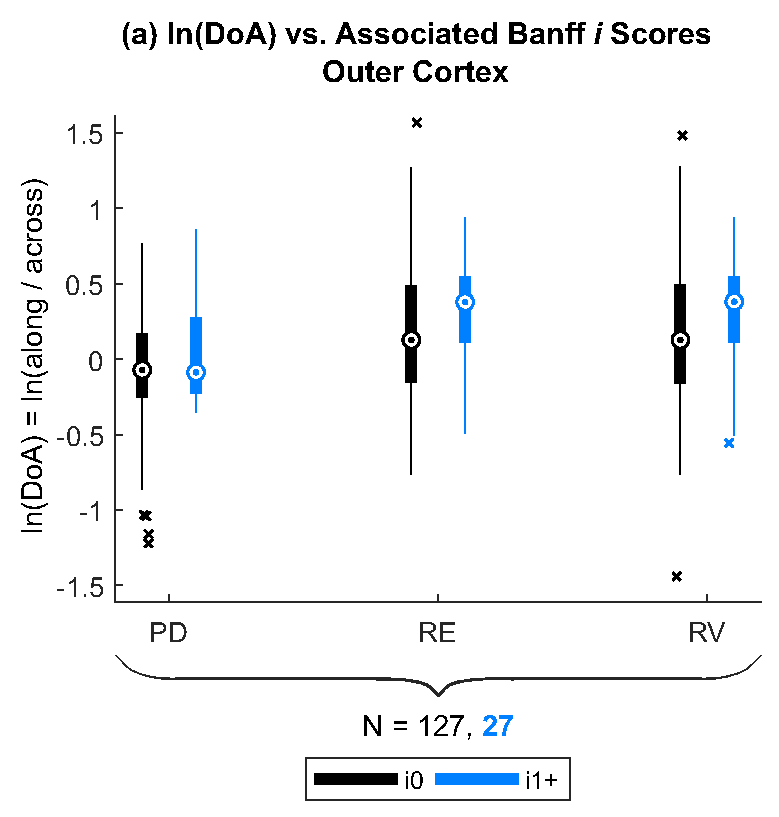
\includegraphics[width=0.24\textwidth]{
            parts/transplant/figs/boxplot-doa/doa-all-i/doa_F1.5_i_oc.eps
        }
        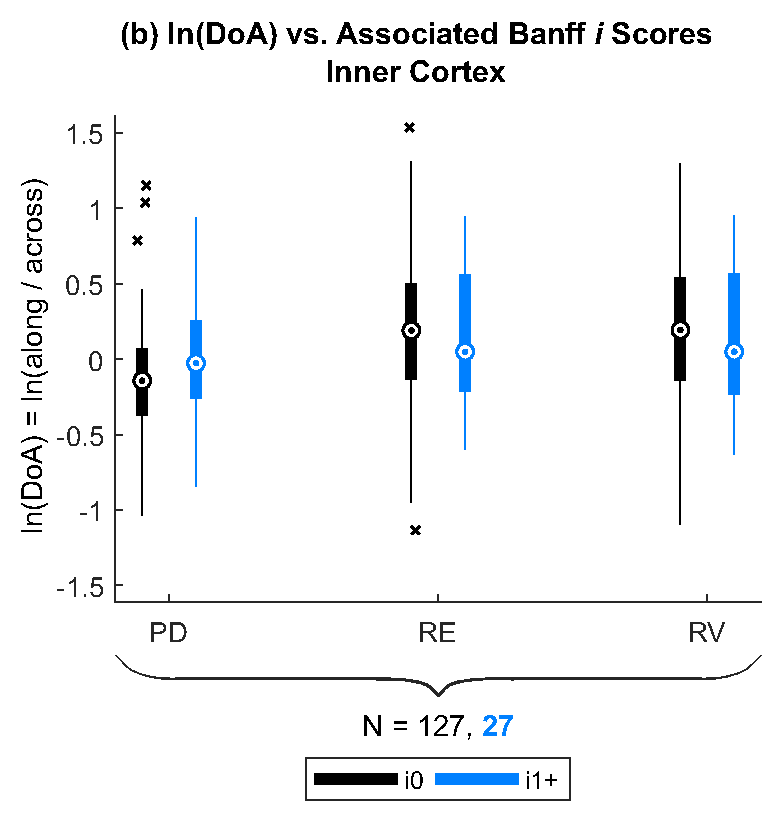
\includegraphics[width=0.24\textwidth]{
            parts/transplant/figs/boxplot-doa/doa-all-i/doa_F1.5_i_ic.eps
        }
        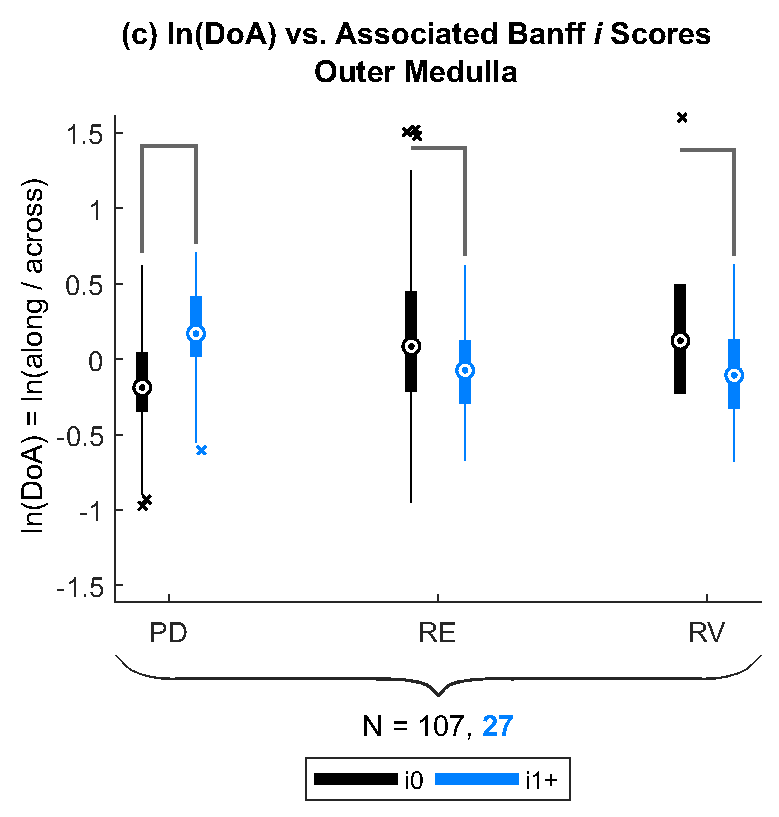
\includegraphics[width=0.24\textwidth]{
            parts/transplant/figs/boxplot-doa/doa-all-i/doa_F1.5_i_om.eps
        }
        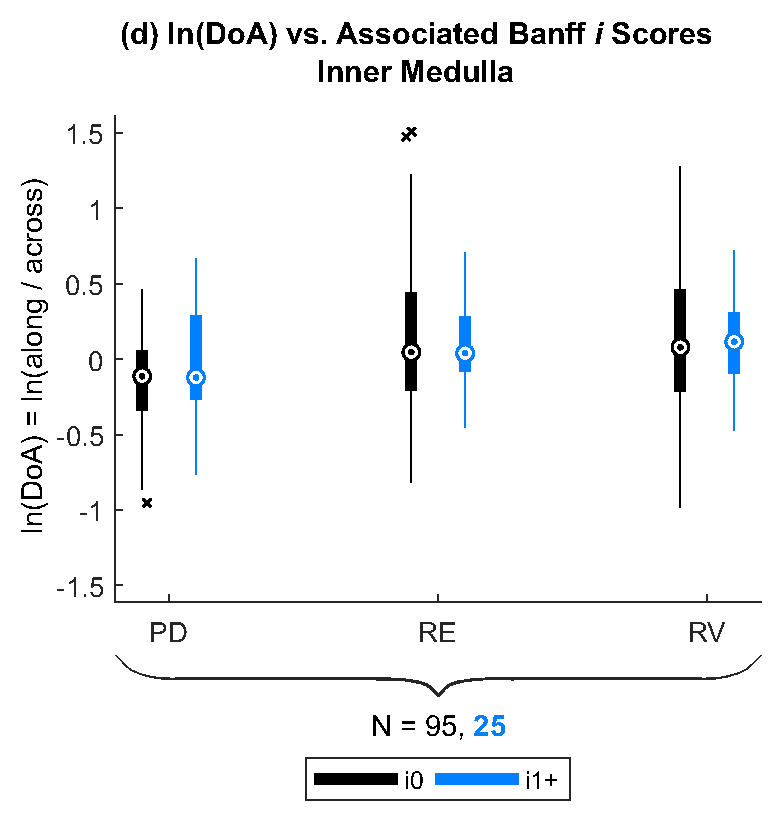
\includegraphics[width=0.24\textwidth]{
            parts/transplant/figs/boxplot-doa/doa-all-i/doa_F1.5_i_im.eps
        }
    \end{subfigure}
    \begin{subfigure}[b]{\textwidth}
        \centering
        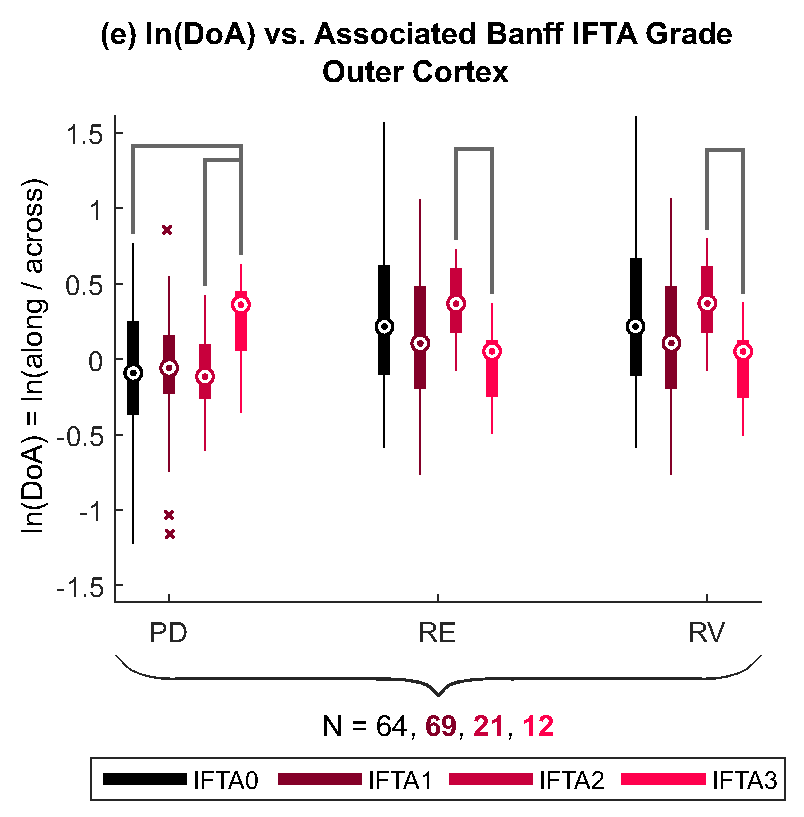
\includegraphics[width=0.24\textwidth]{
            parts/transplant/figs/boxplot-doa/doa-all-ifta/doa_F1.5_ifta_oc.eps
        }
        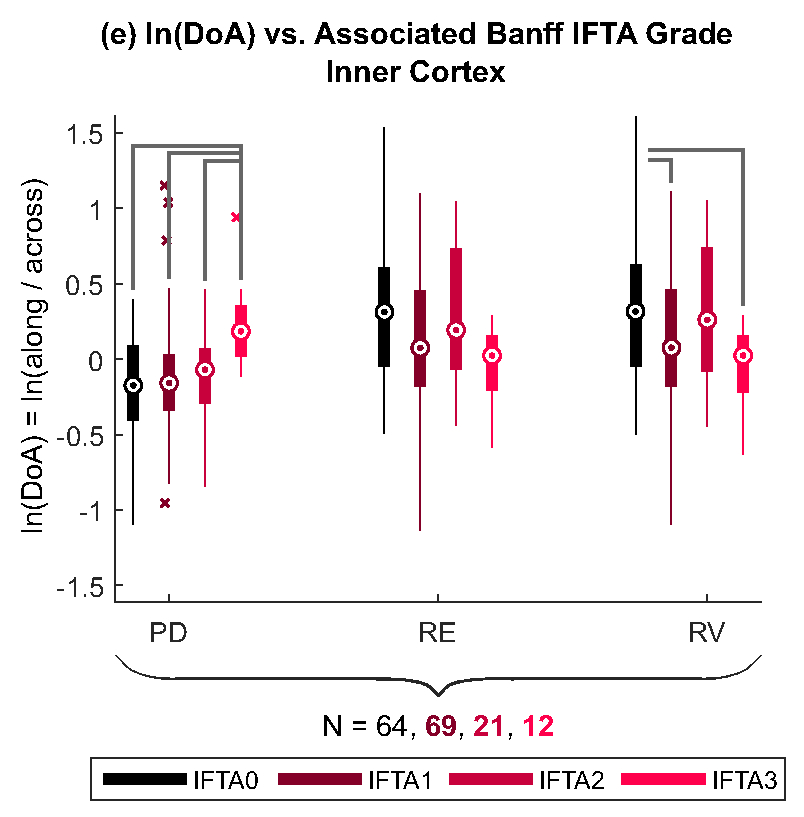
\includegraphics[width=0.24\textwidth]{
            parts/transplant/figs/boxplot-doa/doa-all-ifta/doa_F1.5_ifta_ic.eps
        }
        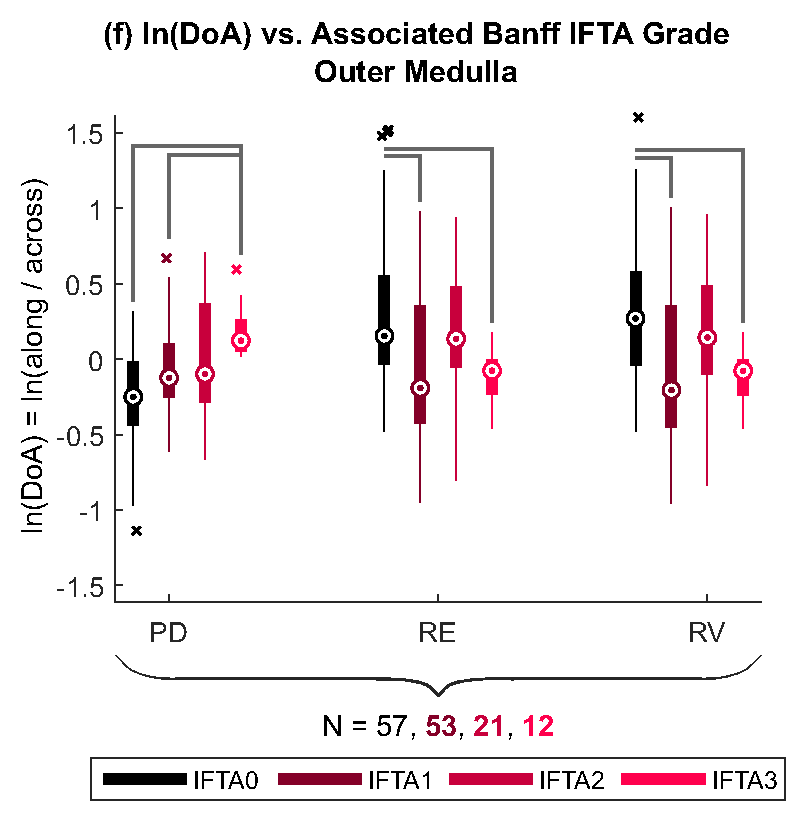
\includegraphics[width=0.24\textwidth]{
            parts/transplant/figs/boxplot-doa/doa-all-ifta/doa_F1.5_ifta_om.eps
        }
        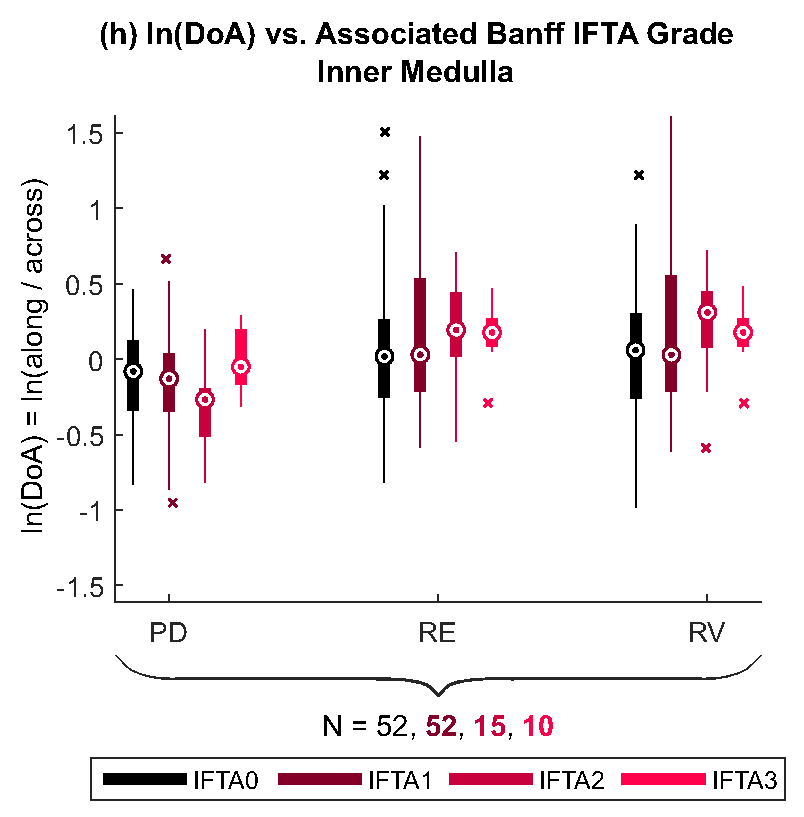
\includegraphics[width=0.24\textwidth]{
            parts/transplant/figs/boxplot-doa/doa-all-ifta/doa_F1.5_ifta_im.eps
        }
    \end{subfigure}
    \begin{subfigure}[b]{\textwidth}
        \centering
        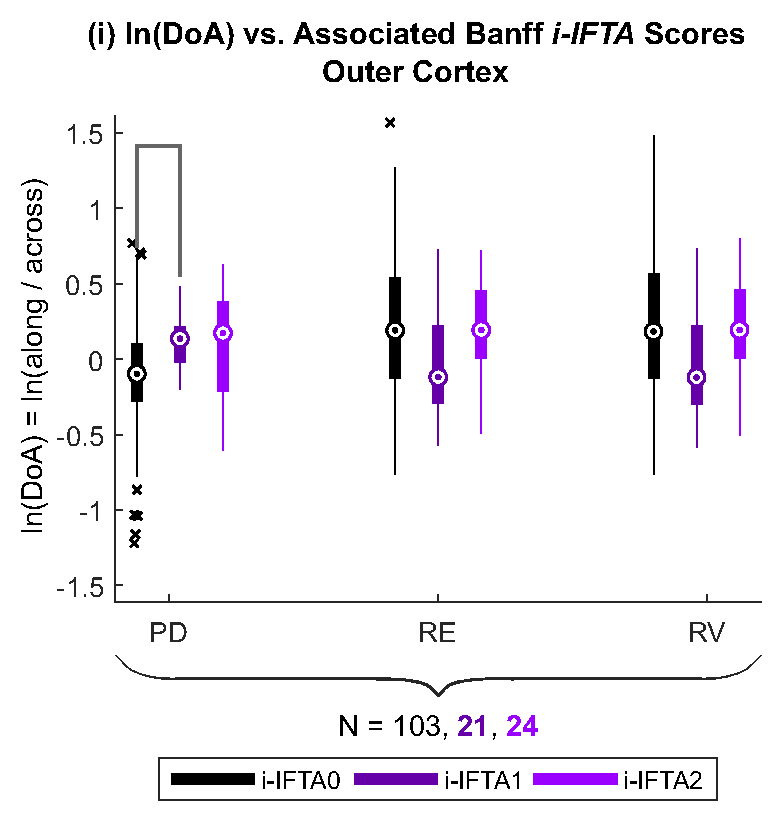
\includegraphics[width=0.24\textwidth]{
            parts/transplant/figs/boxplot-doa/doa-all-i-ifta/doa_F1.5_i-ifta_oc.eps
        }
        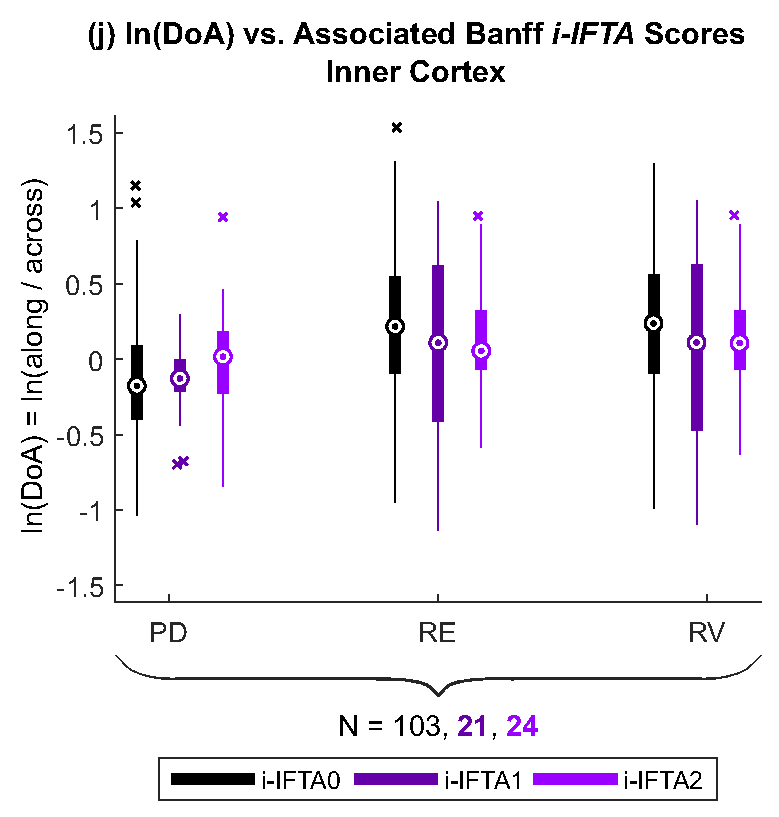
\includegraphics[width=0.24\textwidth]{
            parts/transplant/figs/boxplot-doa/doa-all-i-ifta/doa_F1.5_i-ifta_ic.eps
        }
        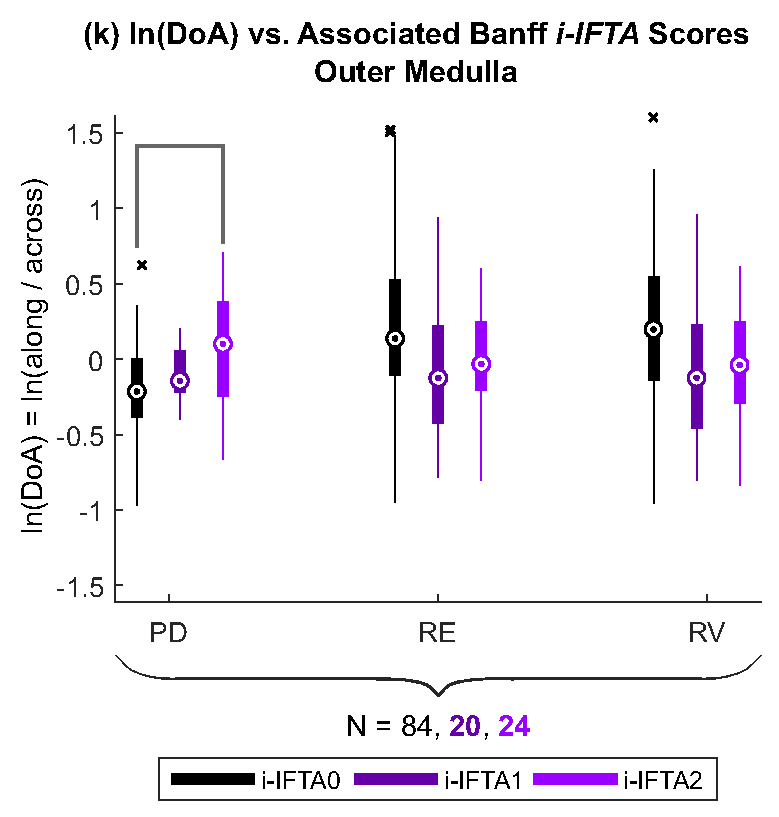
\includegraphics[width=0.24\textwidth]{
            parts/transplant/figs/boxplot-doa/doa-all-i-ifta/doa_F1.5_i-ifta_om.eps
        }
        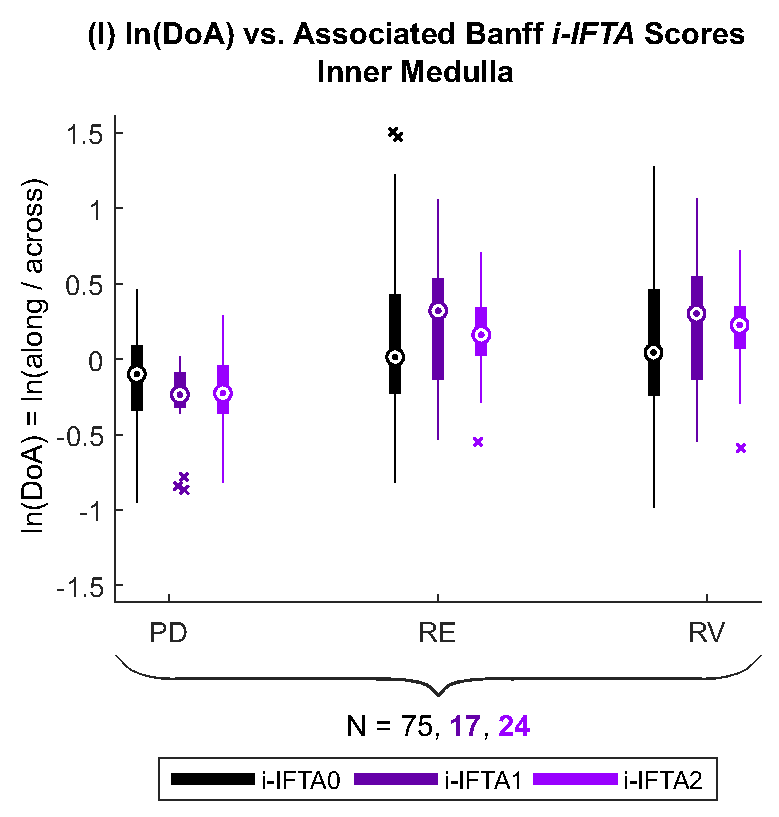
\includegraphics[width=0.24\textwidth]{
            parts/transplant/figs/boxplot-doa/doa-all-i-ifta/doa_F1.5_i-ifta_im.eps
        }
    \end{subfigure}
    \begin{subfigure}[b]{\textwidth}
        \centering
        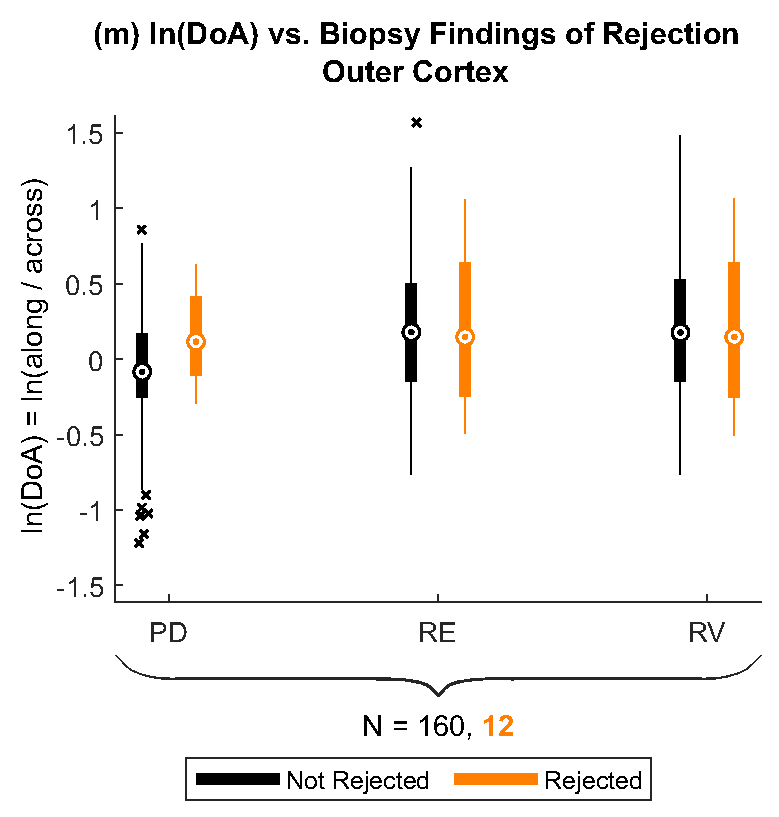
\includegraphics[width=0.24\textwidth]{
            parts/transplant/figs/boxplot-doa/doa-all-reject/doa_F1.5_reject_oc.eps
        }
        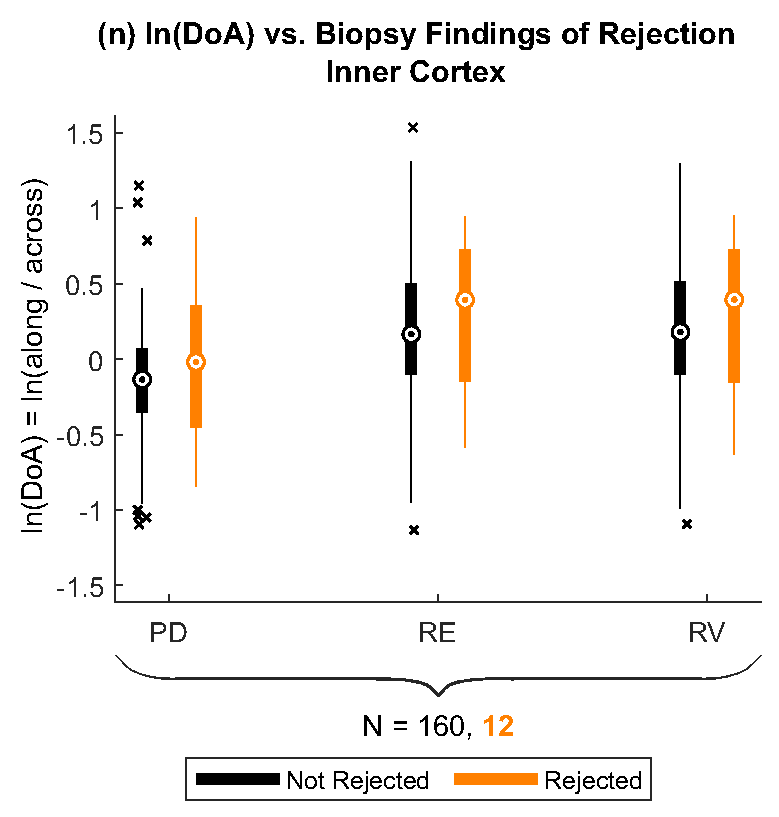
\includegraphics[width=0.24\textwidth]{
            parts/transplant/figs/boxplot-doa/doa-all-reject/doa_F1.5_reject_ic.eps
        }
        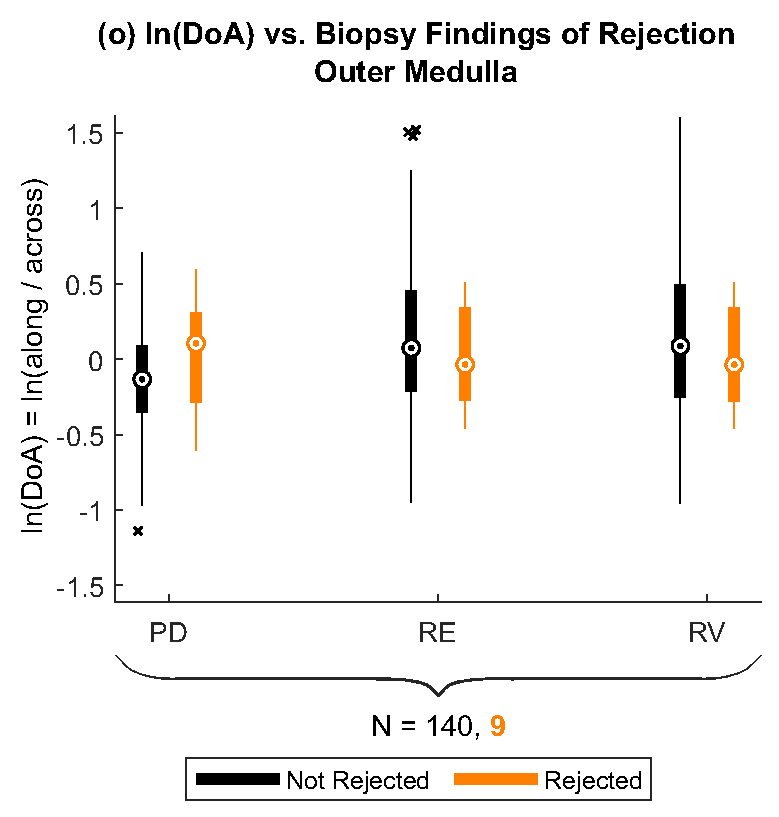
\includegraphics[width=0.24\textwidth]{
            parts/transplant/figs/boxplot-doa/doa-all-reject/doa_F1.5_reject_om.eps
        }
        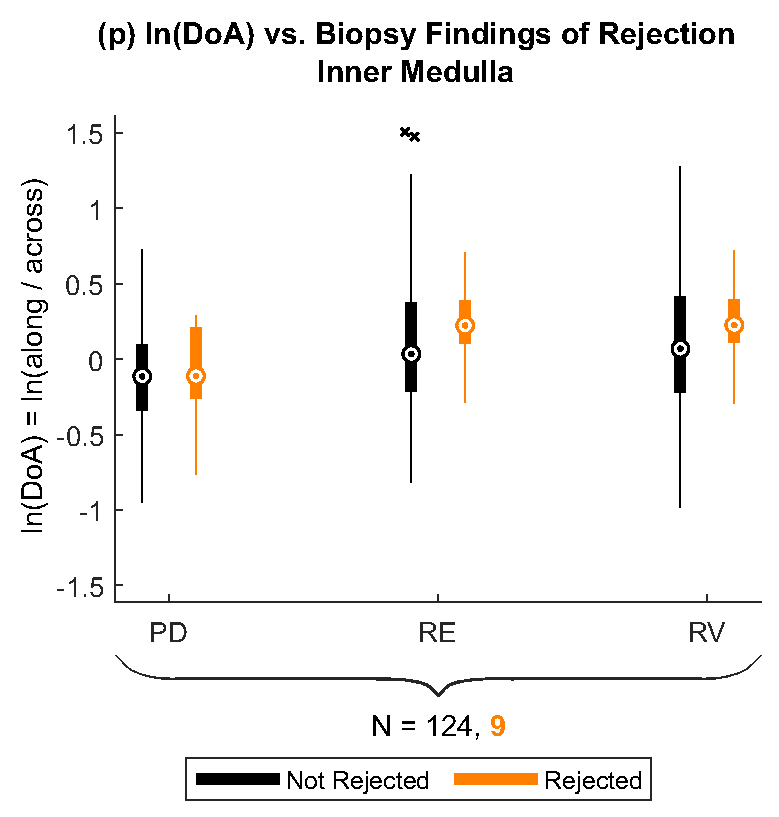
\includegraphics[width=0.24\textwidth]{
            parts/transplant/figs/boxplot-doa/doa-all-reject/doa_F1.5_reject_im.eps
        }
    \end{subfigure}
    \caption{Box plots of DoA based on PD, RE, and RV measurements, grouped by associated biopsy findings of (a--d) \emph{i} (interstitial inflammation) scores, (e--h) IFTA (interstitial fibrosis/tubular atrophy) grading, (i--l) \emph{i-IFTA} (inflammation in areas of IFTA) scores, and (m--p) whether biopsies indicated graft rejection. Values are shown for DoA at the (a,e,i,m) outer cortex, (b,f,j,n) inner cortex, (c,g,k,o) outer medulla, and (d,h,l,p) inner medulla. Numbers written under x-axes denote number of ROIs represented by each distribution. Pairs of box plots connected with gray bars denote statistically significant differences ($p < 0.05$) between biopsy findings based on Kruskal-Wallis test and Bonferroni correction. DoA values without matched biopsy findings are not shown.}
    \label{fig:clinicalVisrDoa}
\end{figure}


% Box plot of PD, RE, RV-based RR strat by i, IFTA, i-IFTA scores, rejection
% !TeX root = ../../../main.tex

% Key observations:
% - direction of change in PD and RE/RV are opposite here, too
% - RE and RV also appear incredibly similar in trends, just like DoA
% - PD, RE, and RV-based DoA are all significantly different in:
%   - IFTA 0 vs 2: outer medulla vs inner medulla
%   - i-IFTA 0 vs 2: outer medulla vs inner medulla
%   - Rejection: outer/inner cortex, outer/inner medulla

\begin{figure}[!tbp]
    \centering
    \begin{subfigure}[b]{\textwidth}
        \centering
        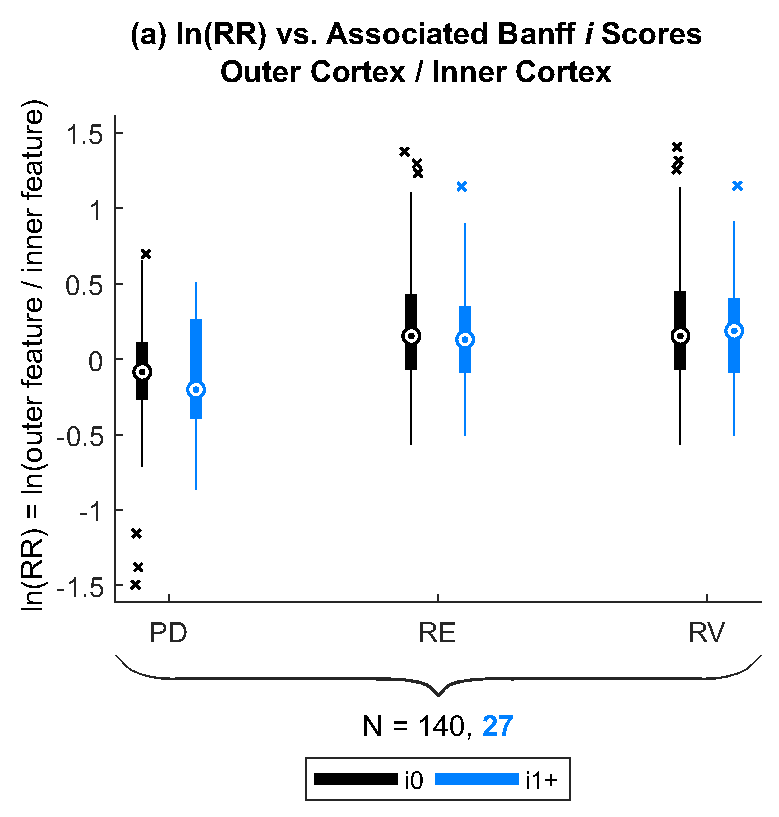
\includegraphics[width=0.24\textwidth]{
            parts/transplant/figs/boxplot-rr/rr-all-i/rr_F1.5_i_oc-ic.eps
        }
        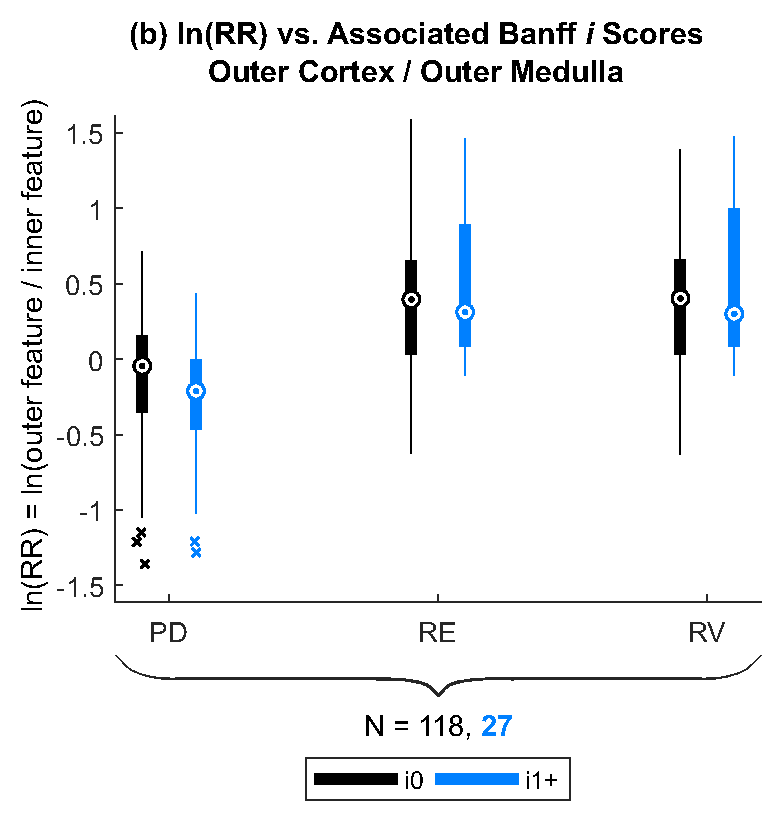
\includegraphics[width=0.24\textwidth]{
            parts/transplant/figs/boxplot-rr/rr-all-i/rr_F1.5_i_oc-om.eps
        }
        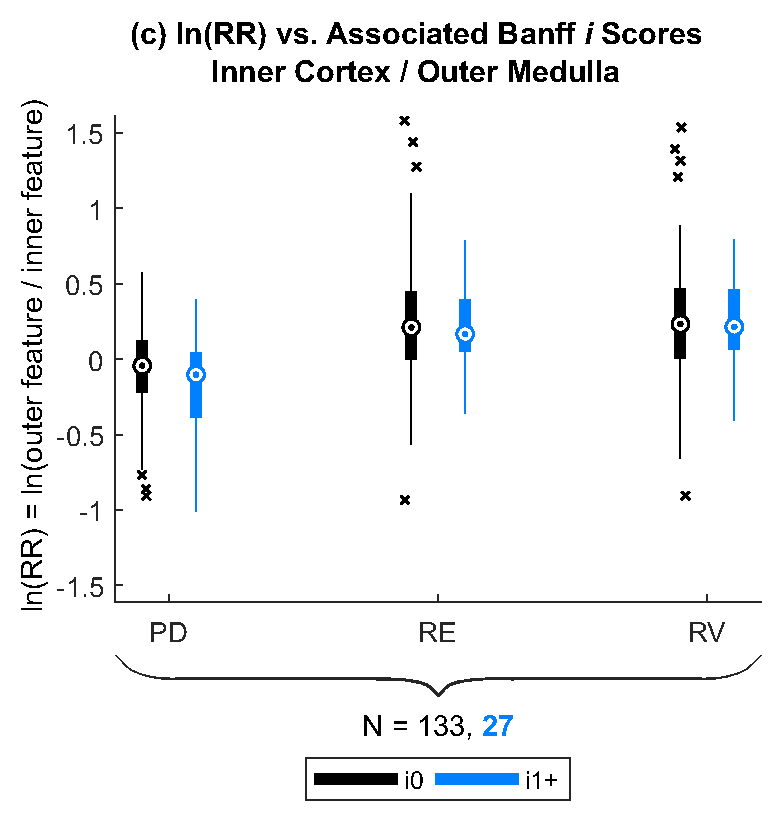
\includegraphics[width=0.24\textwidth]{
            parts/transplant/figs/boxplot-rr/rr-all-i/rr_F1.5_i_ic-om.eps
        }
        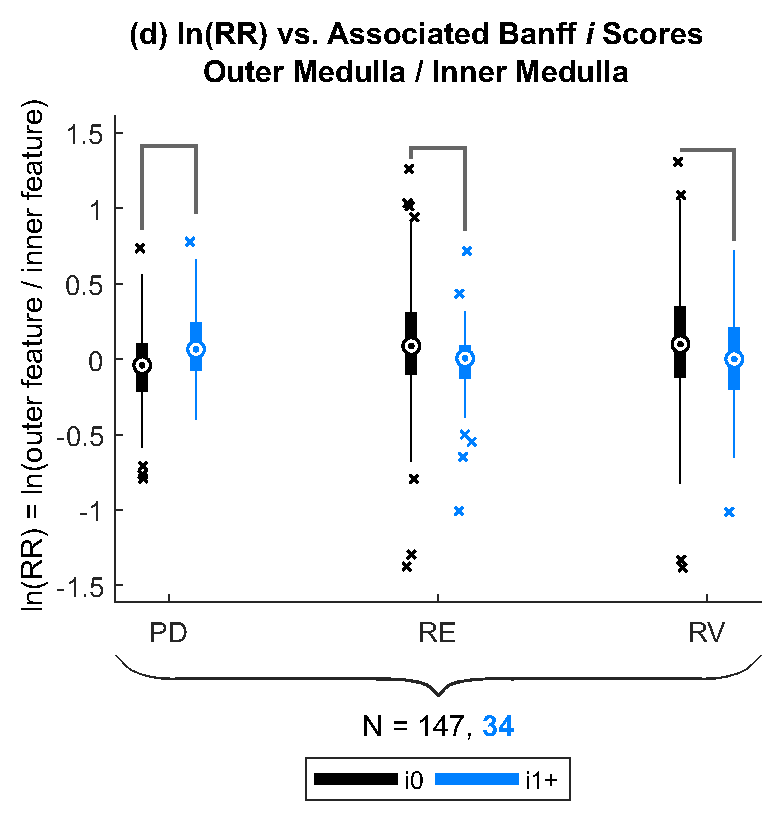
\includegraphics[width=0.24\textwidth]{
            parts/transplant/figs/boxplot-rr/rr-all-i/rr_F1.5_i_om-im.eps
        }
    \end{subfigure}
    \begin{subfigure}[b]{\textwidth}
        \centering
        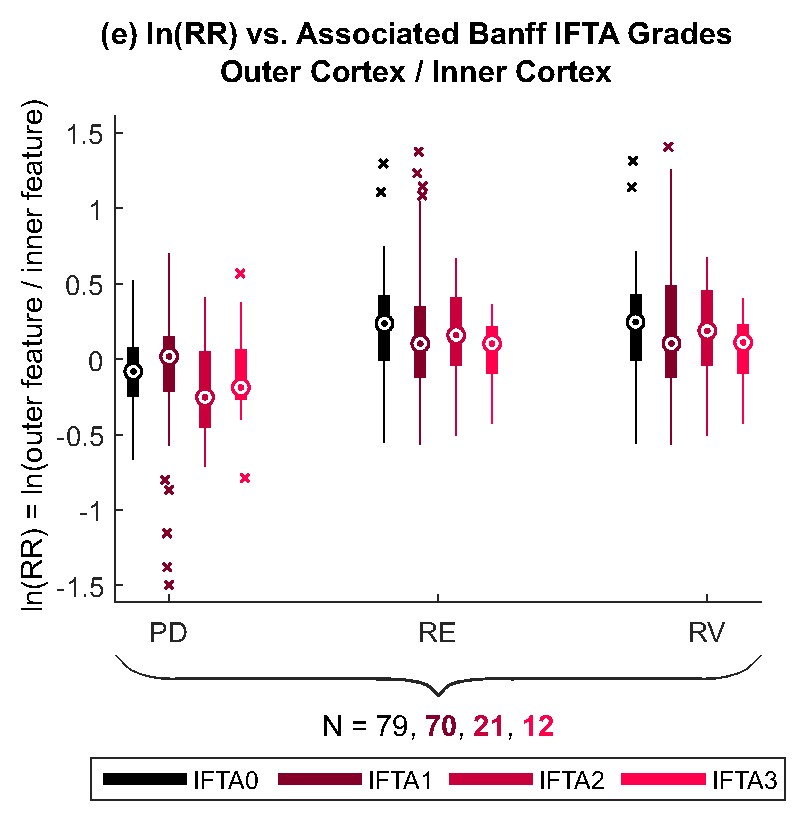
\includegraphics[width=0.24\textwidth]{
            parts/transplant/figs/boxplot-rr/rr-all-ifta/rr_F1.5_ifta_oc-ic.eps
        }
        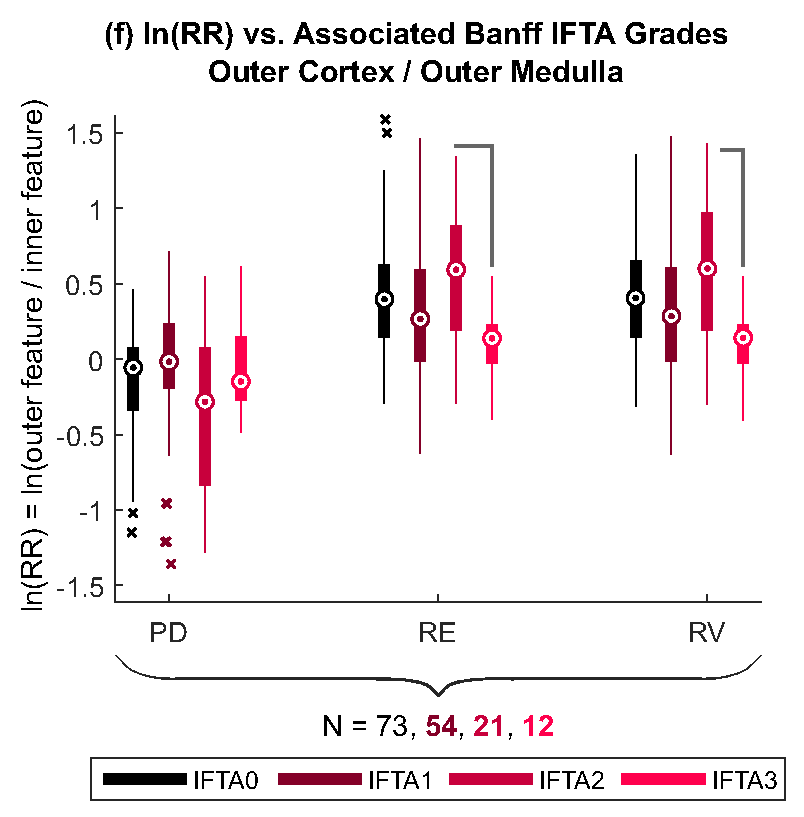
\includegraphics[width=0.24\textwidth]{
            parts/transplant/figs/boxplot-rr/rr-all-ifta/rr_F1.5_ifta_oc-om.eps
        }
        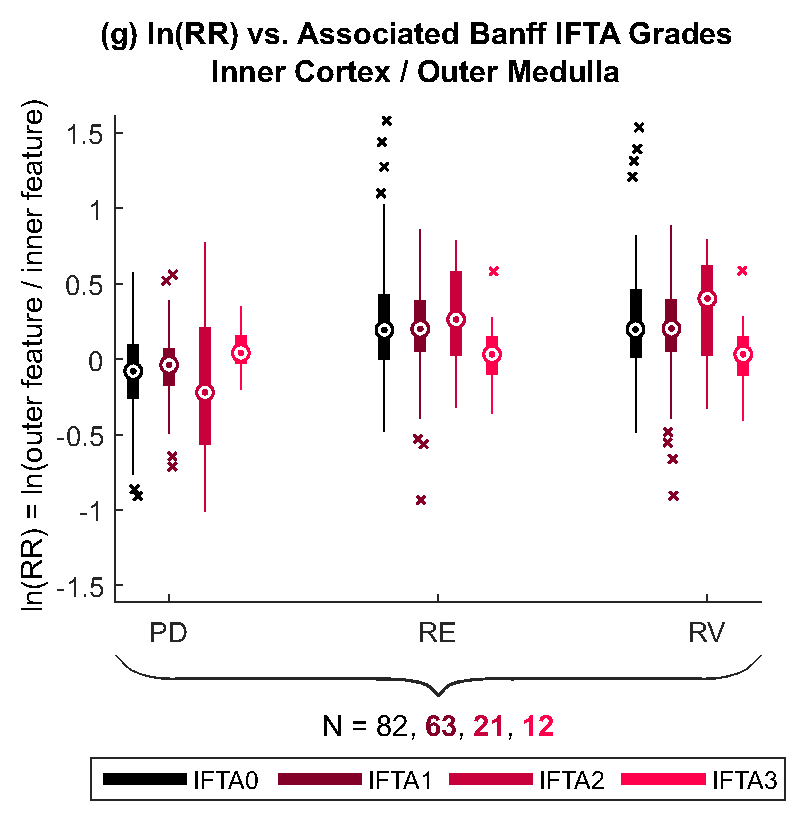
\includegraphics[width=0.24\textwidth]{
            parts/transplant/figs/boxplot-rr/rr-all-ifta/rr_F1.5_ifta_ic-om.eps
        }
        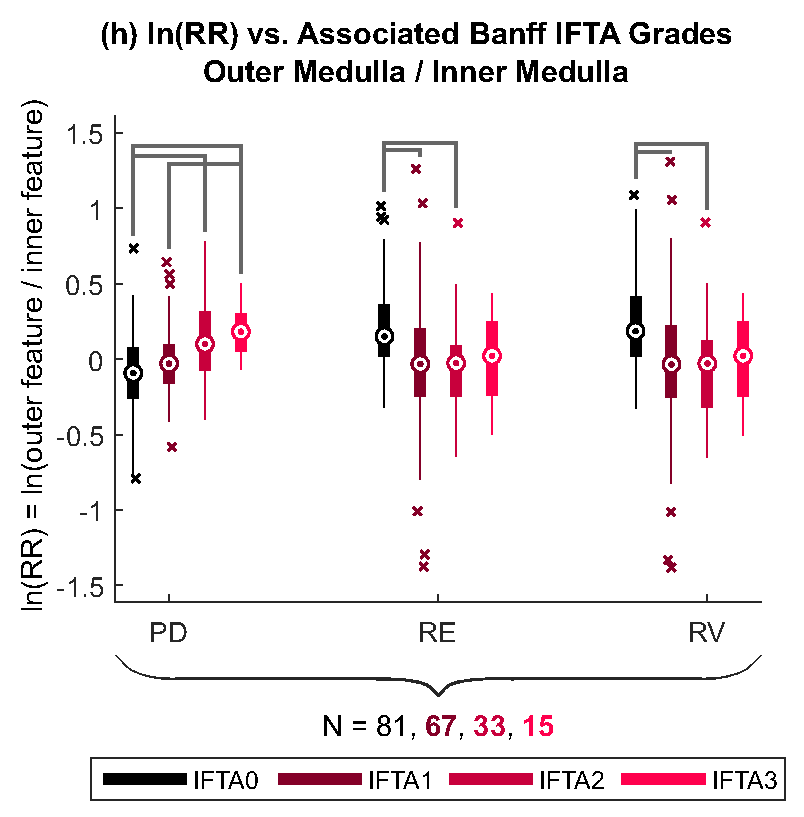
\includegraphics[width=0.24\textwidth]{
            parts/transplant/figs/boxplot-rr/rr-all-ifta/rr_F1.5_ifta_om-im.eps
        }
    \end{subfigure}
    \begin{subfigure}[b]{\textwidth}
        \centering
        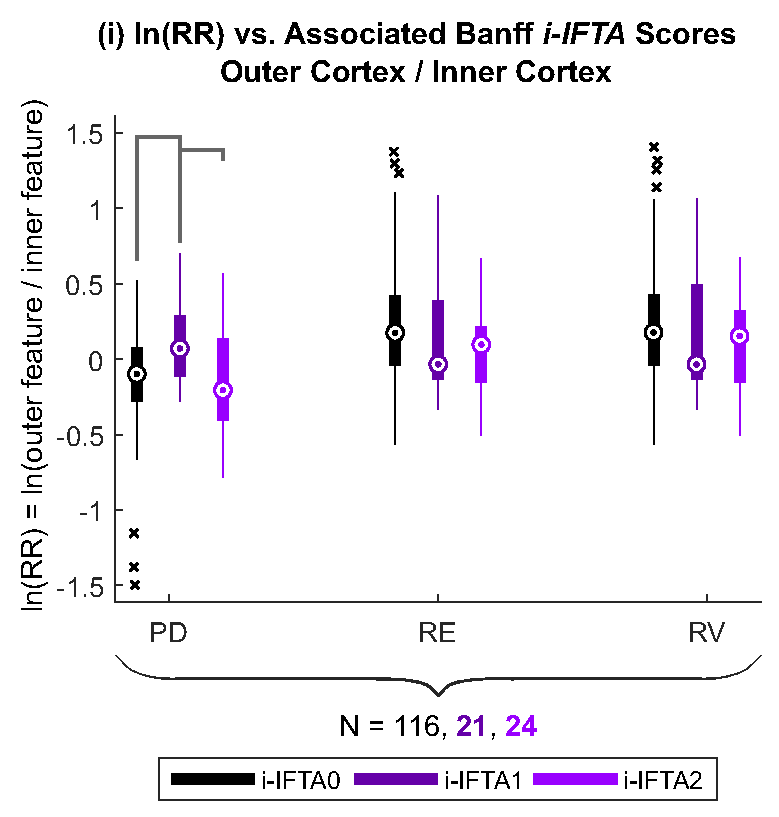
\includegraphics[width=0.24\textwidth]{
            parts/transplant/figs/boxplot-rr/rr-all-i-ifta/rr_F1.5_i-ifta_oc-ic.eps
        }
        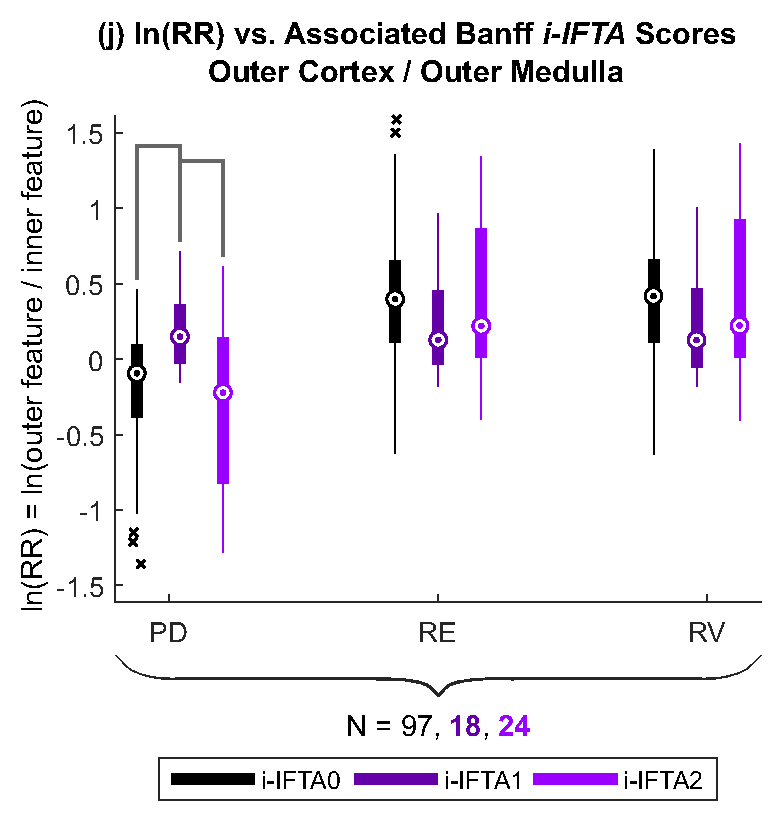
\includegraphics[width=0.24\textwidth]{
            parts/transplant/figs/boxplot-rr/rr-all-i-ifta/rr_F1.5_i-ifta_oc-om.eps
        }
        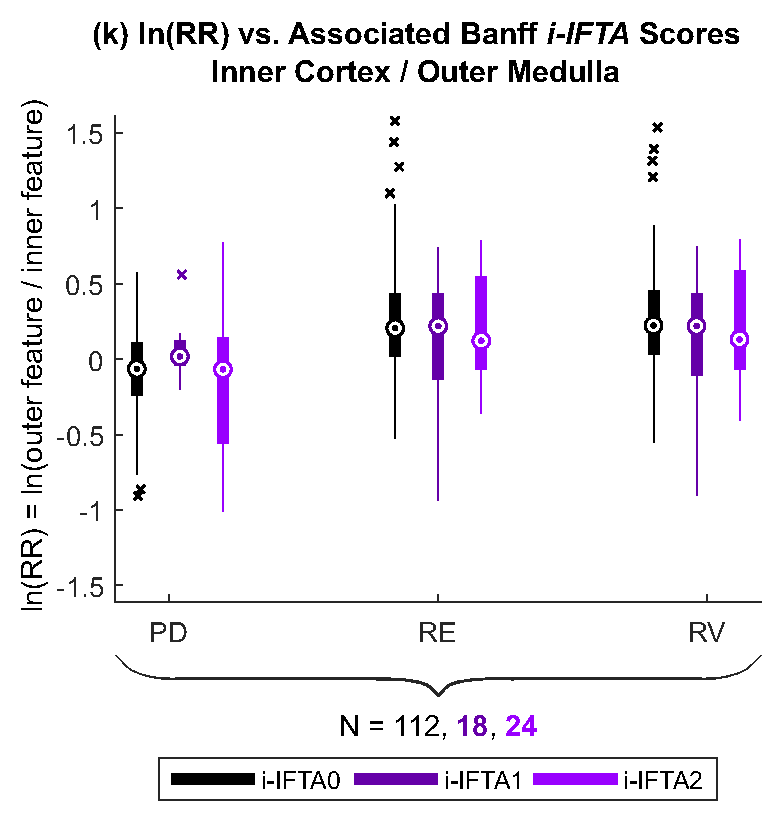
\includegraphics[width=0.24\textwidth]{
            parts/transplant/figs/boxplot-rr/rr-all-i-ifta/rr_F1.5_i-ifta_ic-om.eps
        }
        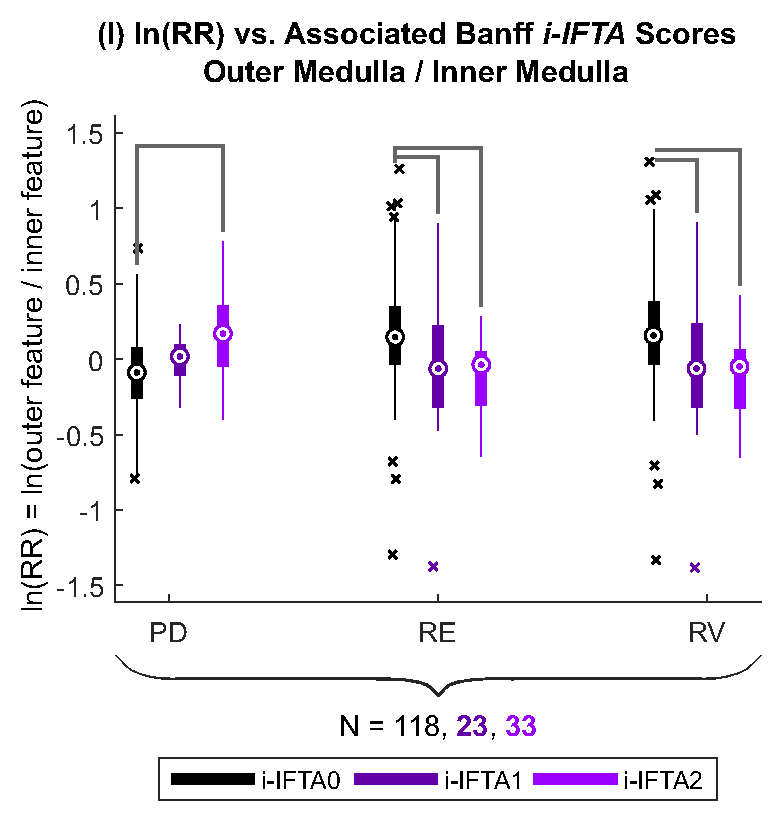
\includegraphics[width=0.24\textwidth]{
            parts/transplant/figs/boxplot-rr/rr-all-i-ifta/rr_F1.5_i-ifta_om-im.eps
        }
    \end{subfigure}
    \begin{subfigure}[b]{\textwidth}
        \centering
        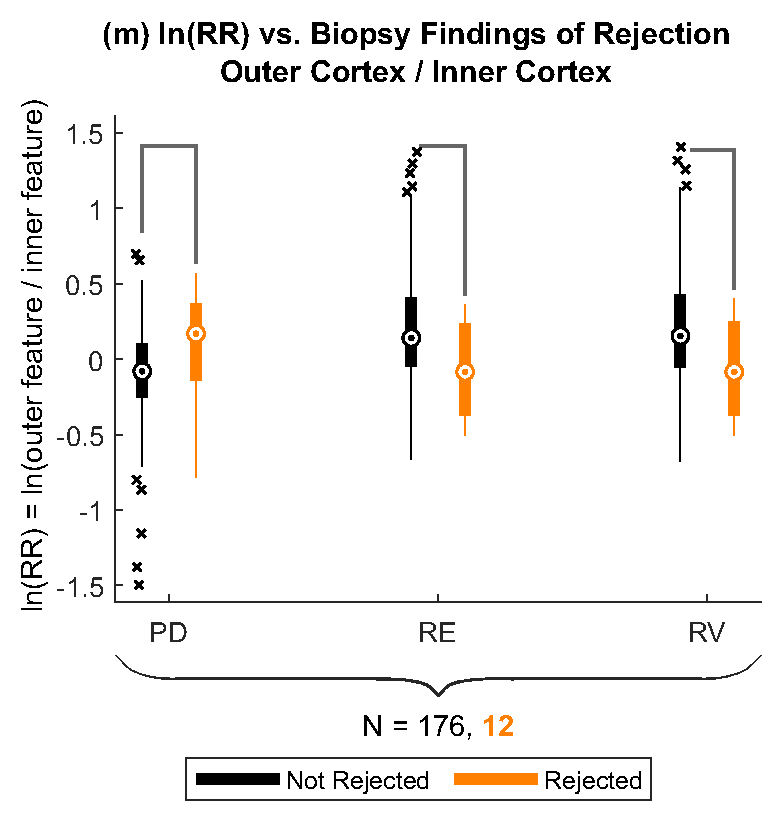
\includegraphics[width=0.24\textwidth]{
            parts/transplant/figs/boxplot-rr/rr-all-reject/rr_F1.5_reject_oc-ic.eps
        }
        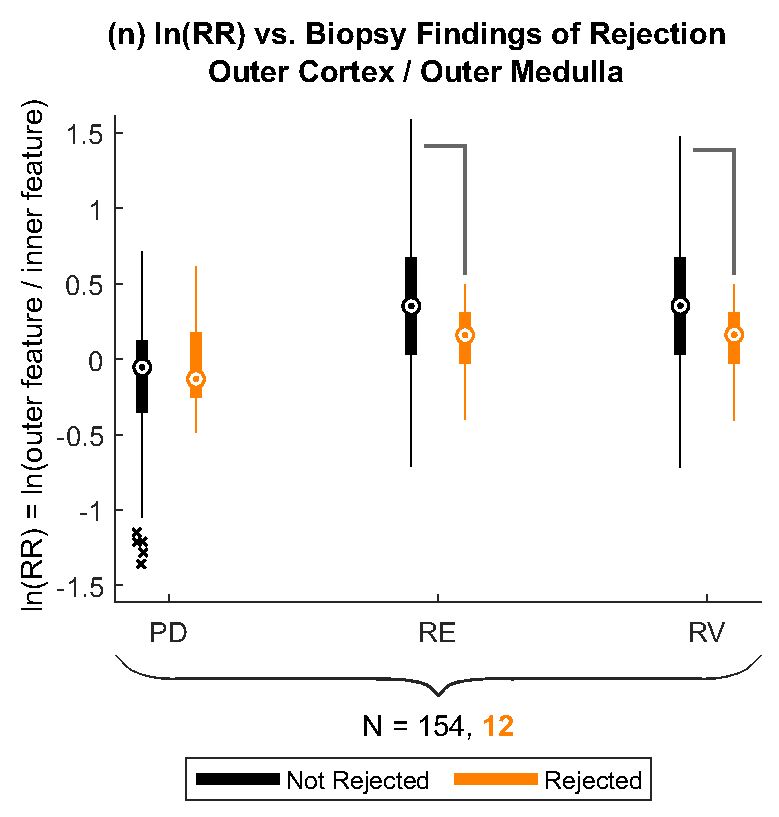
\includegraphics[width=0.24\textwidth]{
            parts/transplant/figs/boxplot-rr/rr-all-reject/rr_F1.5_reject_oc-om.eps
        }
        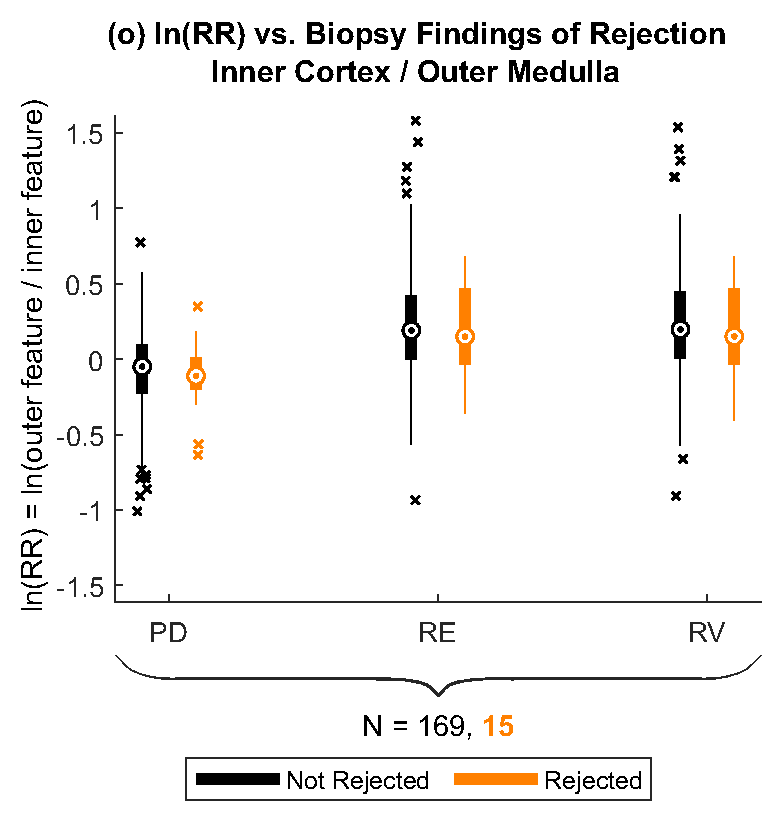
\includegraphics[width=0.24\textwidth]{
            parts/transplant/figs/boxplot-rr/rr-all-reject/rr_F1.5_reject_ic-om.eps
        }
        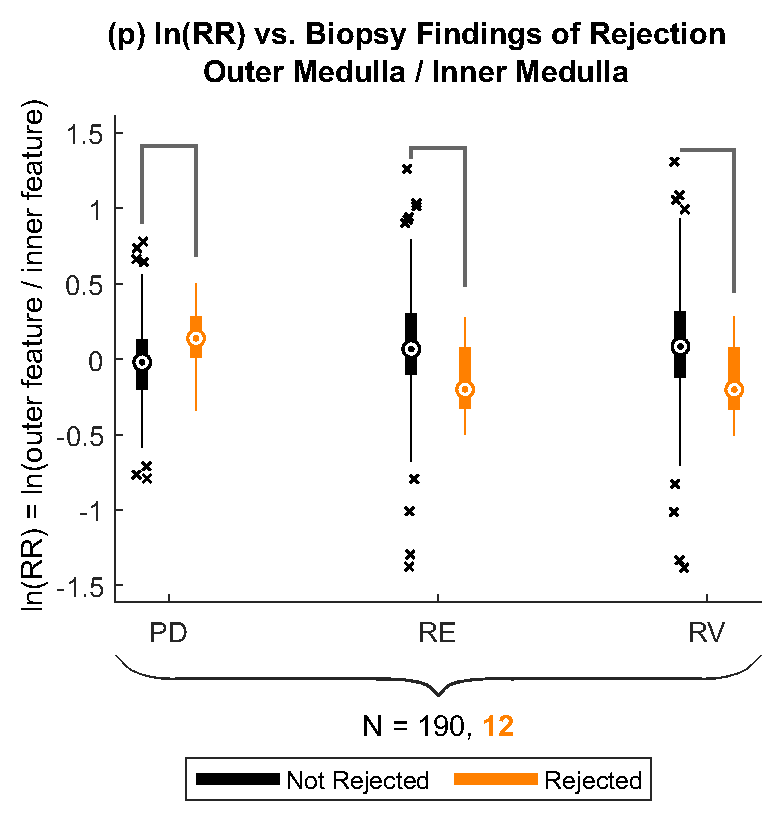
\includegraphics[width=0.24\textwidth]{
            parts/transplant/figs/boxplot-rr/rr-all-reject/rr_F1.5_reject_om-im.eps
        }
    \end{subfigure}
    \caption{Box plots of RR based on PD, RE, and RV measurements, grouped by associated biopsy findings of (a--d) \emph{i} (interstitial inflammation) scores, (e--h) IFTA (interstitial fibrosis/tubular atrophy) grading, (i--l) \emph{i-IFTA} (inflammation in areas of IFTA) scores, and (m--p) whether biopsies indicated graft rejection. Values are shown for RR between the (a,e,i,m) outer versus inner cortex, (b,f,j,n) outer cortex over outer medulla, (c,g,k,o) inner cortex over outer medulla, and (d,h,l,p) outer versus inner medulla. Numbers written under x-axes denote number of ROIs represented by each distribution. Pairs of box plots connected with gray bars denote statistically significant differences ($p < 0.05$) between biopsy findings based on Kruskal-Wallis test and Bonferroni correction. RR values without matched biopsy findings are not shown.}
    \label{fig:clinicalVisrRr}
\end{figure}


Table~\ref{tbl:clinicalRegressor} summarizes the Spearman's rank correlation coefficient and estimation error metrics of regression models that relate clinical variables to VisR-derived DoA and RR metrics. As mentioned previously, only variables that allowed for meaningful regression analyses (i.e. those based on continous scales or ordinal scales with more than two categories) were included. Likewise, Table~\ref{tbl:clinicalClassifier} summarizes the performance metrics of classification models predicting clinical variables from VisR-derived DoA and RR metrics. In both tables, metrics are reported for models trained using PD, RE, and RV metrics separately. Metrics marked with an asterisk (*) indicate the best performing model for each clinical variable.

% Table of regressor performance metrics for clinical variables
\afterpage{%
    \clearpage
    % !TeX root = ../../../main.tex

\begin{landscape}
    \singlespacing
    \centering
    \fontsize{8}{8}\selectfont
    \begin{longtable}{
        p{0.9in} 
        ll w{r}{0.7in} w{r}{0.7in} w{r}{0.7in}
        ll w{r}{0.7in} w{r}{0.7in} w{r}{0.7in}
    }
        \caption{Performance Metrics for Regression Models Predicting Clinical Variables from VisR-Derived Metrics}\\
        \label{tbl:clinicalRegressor}\\
        \toprule
        \multirow{2}{=}{Response Variable} & 
        \multicolumn{5}{c}{DoA} & 
        \multicolumn{5}{c}{RR} \\
        \cmidrule(r){2-6}\cmidrule(r){7-11}
         & Input & Metric & PD & RE & RV &  % secondary heading for DoA
        Input & Metric & PD & RE & RV \\ % secondary heading for RR
        \midrule
        \endfirsthead
        \endhead
        \endlastfoot
        %
        % Serum Creatinine vs VisR metrics
        %
        \multirow{8}{=}{Serum Creatinine} & 
        \multirow{2}{*}{oC} & $\rho_{s}$ & 
        % Spearman's rho for DoA
        \textsuperscript{\textdagger{}}0.10 $\pm$ 0.11 & -0.05 $\pm$ 0.08 & -0.05 $\pm$ 0.07 &
        \multirow{2}{*}{oC/iC} & $\rho_{s}$ & 
        % Spearman's rho for RR
        0.03 $\pm$ 0.15 & 0.00 $\pm$ 0.10 & 0.01 $\pm$ 0.09 \\ 
         & & RMSE &
         % RMSE for DoA
        \textbf{*\textsuperscript{\textdagger{}}0.36 $\pm$ 0.04} & \textbf{*\textsuperscript{\textdagger{}}0.36 $\pm$ 0.04} & \textbf{*\textsuperscript{\textdagger{}}0.36 $\pm$ 0.04} &
         & RMSE &
        % RMSE for RR
        \textbf{*\textsuperscript{\textdagger{}}0.36 $\pm$ 0.05} & \textbf{*\textsuperscript{\textdagger{}}0.36 $\pm$ 0.05} & \textbf{*\textsuperscript{\textdagger{}}0.36 $\pm$ 0.05} \\ 
        \cmidrule{2-11} & \multirow{2}{*}{iC} & $\rho_{s}$ & 
        % Spearman's rho for DoA
        0.08 $\pm$ 0.13 & -0.05 $\pm$ 0.08 & -0.04 $\pm$ 0.08 &
        \multirow{2}{*}{oC/oM} & $\rho_{s}$ & 
        % Spearman's rho for RR
        -0.02 $\pm$ 0.09 & -0.00 $\pm$ 0.09 & -0.00 $\pm$ 0.09 \\ 
         & & RMSE &
        % RMSE for DoA
        \textbf{*\textsuperscript{\textdagger{}}0.37 $\pm$ 0.05} & \textbf{*\textsuperscript{\textdagger{}}0.37 $\pm$ 0.05} & \textbf{*\textsuperscript{\textdagger{}}0.37 $\pm$ 0.05} &
         & RMSE &
        % RMSE for RR
        \textbf{*\textsuperscript{\textdagger{}}0.37 $\pm$ 0.05} & \textbf{*\textsuperscript{\textdagger{}}0.37 $\pm$ 0.05} & \textbf{*\textsuperscript{\textdagger{}}0.37 $\pm$ 0.05} \\ 
        \cmidrule{2-11} & \multirow{2}{*}{oM} & $\rho_{s}$ & 
        % Spearman's rho for DoA
        0.06 $\pm$ 0.17 & -0.03 $\pm$ 0.12 & -0.03 $\pm$ 0.12 & 
        \multirow{2}{*}{iC/oM} & $\rho_{s}$ & 
        % Spearman's rho for RR
        -0.03 $\pm$ 0.10 & -0.04 $\pm$ 0.11 & -0.03 $\pm$ 0.11 \\ 
         & & RMSE &
        % RMSE for DoA
        \textbf{*\textsuperscript{\textdagger{}}0.38 $\pm$ 0.05} & \textbf{*\textsuperscript{\textdagger{}}0.38 $\pm$ 0.05} & \textbf{*\textsuperscript{\textdagger{}}0.38 $\pm$ 0.05} & 
         & RMSE &
        % RMSE for RR
        \textbf{*\textsuperscript{\textdagger{}}0.36 $\pm$ 0.06} & \textbf{*\textsuperscript{\textdagger{}}0.36 $\pm$ 0.06} & \textbf{*\textsuperscript{\textdagger{}}0.36 $\pm$ 0.06} \\ 
        \cmidrule{2-11} & \multirow{2}{*}{iM} & $\rho_{s}$ & 
        % Spearman's rho for DoA
        0.00 $\pm$ 0.17 & 0.03 $\pm$ 0.18 & 0.04 $\pm$ 0.18 & 
        \multirow{2}{*}{oM/iM} & $\rho_{s}$ & 
        % Spearman's rho for RR
        -0.02 $\pm$ 0.11 & -0.07 $\pm$ 0.11 & \textsuperscript{\textdagger{}}-0.08 $\pm$ 0.10 \\ 
         & & RMSE &
        % RMSE for DoA
        \textsuperscript{\textdagger{}}0.39 $\pm$ 0.07 & \textsuperscript{\textdagger{}}0.39 $\pm$ 0.07 & \textsuperscript{\textdagger{}}0.39 $\pm$ 0.07 & 
         & RMSE &
        % RMSE for RR
        \textbf{*\textsuperscript{\textdagger{}}0.38 $\pm$ 0.04} & \textbf{*\textsuperscript{\textdagger{}}0.38 $\pm$ 0.04} & \textbf{*\textsuperscript{\textdagger{}}0.38 $\pm$ 0.04} \\ 
        \midrule
        %
        % UPCR vs VisR metrics
        %
        \multirow{8}{=}{UPCR} & 
        \multirow{2}{*}{oC} & $\rho_{s}$ & 
        % Spearman's rho for DoA
        0.05 $\pm$ 0.12 & -0.02 $\pm$ 0.11 & -0.02 $\pm$ 0.10 & 
        \multirow{2}{*}{oC/iC} & $\rho_{s}$ & 
        % Spearman's rho for RR
        -0.04 $\pm$ 0.13 & 0.02 $\pm$ 0.11 & 0.02 $\pm$ 0.11 \\ 
         & & RMSE &
        % RMSE for DoA
        \textbf{*\textsuperscript{\textdagger{}}0.58 $\pm$ 0.22} & \textbf{*\textsuperscript{\textdagger{}}0.58 $\pm$ 0.22} & \textbf{*\textsuperscript{\textdagger{}}0.58 $\pm$ 0.22} & 
         & RMSE &
        % RMSE for RR
        \textbf{*\textsuperscript{\textdagger{}}0.59 $\pm$ 0.17} & \textbf{*\textsuperscript{\textdagger{}}0.59 $\pm$ 0.17} & \textbf{*\textsuperscript{\textdagger{}}0.59 $\pm$ 0.17} \\ 
        \cmidrule{2-11} & \multirow{2}{*}{iC} & $\rho_{s}$ & 
        % Spearman's rho for DoA
        \textsuperscript{\textdagger{}}0.08 $\pm$ 0.09 & -0.05 $\pm$ 0.10 & -0.05 $\pm$ 0.10 & 
        \multirow{2}{*}{oC/oM} & $\rho_{s}$ & 
        % Spearman's rho for RR
        \textsuperscript{\textdagger{}}-0.11 $\pm$ 0.11 & 0.06 $\pm$ 0.16 & 0.06 $\pm$ 0.16 \\ 
         & & RMSE &
        % RMSE for DoA
        \textsuperscript{\textdagger{}}0.55 $\pm$ 0.27 & \textsuperscript{\textdagger{}}0.55 $\pm$ 0.27 & \textsuperscript{\textdagger{}}0.56 $\pm$ 0.27 & 
         & RMSE &
        % RMSE for RR
        \textsuperscript{\textdagger{}}0.59 $\pm$ 0.26 & \textsuperscript{\textdagger{}}0.59 $\pm$ 0.26 & \textsuperscript{\textdagger{}}0.59 $\pm$ 0.26 \\ 
        \cmidrule{2-11} & \multirow{2}{*}{oM} & $\rho_{s}$ & 
        % Spearman's rho for DoA
        \textbf{*\textsuperscript{\textdagger{}}0.18 $\pm$ 0.11} & -0.01 $\pm$ 0.15 & -0.03 $\pm$ 0.15 & 
        \multirow{2}{*}{iC/oM} & $\rho_{s}$ & 
        % Spearman's rho for RR
        -\textsuperscript{\textdagger{}}-0.14 $\pm$ 0.12 & 0.06 $\pm$ 0.11 & 0.06 $\pm$ 0.11 \\ 
         & & RMSE &
        % RMSE for DoA
        \textsuperscript{\textdagger{}}0.59 $\pm$ 0.22 & \textsuperscript{\textdagger{}}0.60 $\pm$ 0.23 & \textsuperscript{\textdagger{}}0.60 $\pm$ 0.23 & 
         & RMSE &
        % RMSE for RR
        \textbf{*\textsuperscript{\textdagger{}}0.59 $\pm$ 0.23} & \textbf{*\textsuperscript{\textdagger{}}0.59 $\pm$ 0.23} & \textbf{*\textsuperscript{\textdagger{}}0.59 $\pm$ 0.23} \\ 
        \cmidrule{2-11} & \multirow{2}{*}{iM} & $\rho_{s}$ & 
        % Spearman's rho for DoA
        0.03 $\pm$ 0.10 & -0.06 $\pm$ 0.13 & -0.06 $\pm$ 0.14 & 
        \multirow{2}{*}{oM/iM} & $\rho_{s}$ & 
        % Spearman's rho for RR
        \textbf{*\textsuperscript{\textdagger{}}0.12 $\pm$ 0.07} & 0.00 $\pm$ 0.10 & 0.00 $\pm$ 0.09 \\ 
         & & RMSE &
        % RMSE for DoA
        0.58 $\pm$ 0.23 & 0.58 $\pm$ 0.23 & 0.58 $\pm$ 0.23 & 
         & RMSE &
        % RMSE for RR
        \textbf{*\textsuperscript{\textdagger{}}0.57 $\pm$ 0.18} & \textbf{*\textsuperscript{\textdagger{}}0.58 $\pm$ 0.18} & \textbf{*\textsuperscript{\textdagger{}}0.57 $\pm$ 0.18} \\ 
        \midrule
        %
        % Banff IFTA severity vs VisR metrics
        %
        \multirow{8}{=}{IFTA Grade} & 
        \multirow{2}{*}{oC} & $\rho_{s}$ & 
        % Spearman's rho for DoA
        0.14 $\pm$ 0.26 & -0.10 $\pm$ 0.24 & -0.10 $\pm$ 0.24 &
        \multirow{2}{*}{oC/iC} & $\rho_{s}$ & 
        % Spearman's rho for RR
        -0.04 $\pm$ 0.19 & -0.09 $\pm$ 0.25 & -0.08 $\pm$ 0.25 \\ 
         & & $\mathscr{L_{\textrm{CE}}}$ &
        % Cross-entropy loss for DoA
        \textbf{*\textsuperscript{\textdagger{}}1.19 $\pm$ 0.11} & \textbf{*\textsuperscript{\textdagger{}}1.19 $\pm$ 0.11} & \textbf{*\textsuperscript{\textdagger{}}1.19 $\pm$ 0.11} & 
         & $\mathscr{L_{\textrm{CE}}}$ &
        % Cross-entropy loss for RR
        \textbf{*\textsuperscript{\textdagger{}}1.18 $\pm$ 0.14} & \textbf{*\textsuperscript{\textdagger{}}1.18 $\pm$ 0.14} & \textbf{*\textsuperscript{\textdagger{}}1.18 $\pm$ 0.14} \\ 
        \cmidrule{2-11} & \multirow{2}{*}{iC} & $\rho_{s}$ & 
        % Spearman's rho for DoA
        \textbf{*\textsuperscript{\textdagger{}}0.23 $\pm$ 0.18} & \textbf{*\textsuperscript{\textdagger{}}-0.18 $\pm$ 0.13} & \textbf{*\textsuperscript{\textdagger{}}-0.19 $\pm$ 0.13} & 
        \multirow{2}{*}{oC/oM} & $\rho_{s}$ & 
        % Spearman's rho for RR
        0.02 $\pm$ 0.17 & -0.11 $\pm$ 0.23 & -0.12 $\pm$ 0.24 \\ 
         & & $\mathscr{L_{\textrm{CE}}}$ &
        % Cross-entropy loss for DoA
        \textbf{*\textsuperscript{\textdagger{}}1.18 $\pm$ 0.13} & \textbf{*\textsuperscript{\textdagger{}}1.18 $\pm$ 0.12} & \textbf{*\textsuperscript{\textdagger{}}1.18 $\pm$ 0.12} & 
         & $\mathscr{L_{\textrm{CE}}}$ &
        % Cross-entropy loss for RR
        \textbf{*\textsuperscript{\textdagger{}}1.21 $\pm$ 0.15} & \textbf{*\textsuperscript{\textdagger{}}1.21 $\pm$ 0.14} & \textbf{*\textsuperscript{\textdagger{}}1.21 $\pm$ 0.14} \\ 
        \cmidrule{2-11} & \multirow{2}{*}{oM} & $\rho_{s}$ & 
        % Spearman's rho for DoA
        \textbf{*\textsuperscript{\textdagger{}}0.34 $\pm$ 0.22} & -0.17 $\pm$ 0.34 & -0.17 $\pm$ 0.33 & 
        \multirow{2}{*}{iC/oM} & $\rho_{s}$ & 
        % Spearman's rho for RR
        0.04 $\pm$ 0.19 & -0.04 $\pm$ 0.31 & -0.03 $\pm$ 0.33 \\ 
         & & $\mathscr{L_{\textrm{CE}}}$ &
        % Cross-entropy loss for DoA
        \textsuperscript{\textdagger{}}1.19 $\pm$ 0.18 & \textsuperscript{\textdagger{}}1.24 $\pm$ 0.16 & \textsuperscript{\textdagger{}}1.23 $\pm$ 0.16 & 
         & $\mathscr{L_{\textrm{CE}}}$ &
        % Cross-entropy loss for RR
        \textbf{*\textsuperscript{\textdagger{}}1.19 $\pm$ 0.10} & \textbf{*\textsuperscript{\textdagger{}}1.18 $\pm$ 0.10} & \textbf{*\textsuperscript{\textdagger{}}1.18 $\pm$ 0.10} \\ 
        \cmidrule{2-11} & \multirow{2}{*}{iM} & $\rho_{s}$ & 
        % Spearman's rho for DoA
        -0.08 $\pm$ 0.22 & 0.10 $\pm$ 0.31 & 0.10 $\pm$ 0.30 & 
        \multirow{2}{*}{oM/iM} & $\rho_{s}$ & 
        % Spearman's rho for RR
        \textbf{*\textsuperscript{\textdagger{}}0.38 $\pm$ 0.17} & \textbf{*\textsuperscript{\textdagger{}}-0.34 $\pm$ 0.26} & \textbf{*\textsuperscript{\textdagger{}}-0.34 $\pm$ 0.25} \\ 
         & & $\mathscr{L_{\textrm{CE}}}$ &
        % Cross-entropy loss for DoA
        \textbf{*\textsuperscript{\textdagger{}}1.20 $\pm$ 0.13} & \textbf{*\textsuperscript{\textdagger{}}1.19 $\pm$ 0.14} & \textbf{*\textsuperscript{\textdagger{}}1.19 $\pm$ 0.14} & 
         & $\mathscr{L_{\textrm{CE}}}$ &
        % Cross-entropy loss for RR
        \textbf{*\textsuperscript{\textdagger{}}1.19 $\pm$ 0.10} & \textbf{*\textsuperscript{\textdagger{}}1.21 $\pm$ 0.14} & \textbf{*\textsuperscript{\textdagger{}}1.20 $\pm$ 0.15} \\ 
        \midrule
        %
        % Banff i-IFTA score vs VisR metrics
        %
        \multirow{8}{=}{\textit{i-IFTA} Score} & 
        \multirow{2}{*}{oC} & $\rho_{s}$ & 
        % Spearman's rho for DoA
        \textsuperscript{\textdagger{}}0.24 $\pm$ 0.30 & -0.05 $\pm$ 0.27 & -0.05 $\pm$ 0.27 & 
        \multirow{2}{*}{oC/iC} & $\rho_{s}$ & 
        % Spearman's rho for RR
        0.07 $\pm$ 0.30 & -0.16 $\pm$ 0.26 & -0.10 $\pm$ 0.31 \\ 
         & & $\mathscr{L_{\textrm{CE}}}$ &
        % Cross-entropy loss for DoA
        \textbf{*\textsuperscript{\textdagger{}}0.82 $\pm$ 0.17} & \textbf{*\textsuperscript{\textdagger{}}0.84 $\pm$ 0.14} & \textbf{*\textsuperscript{\textdagger{}}0.84 $\pm$ 0.14} & 
         & $\mathscr{L_{\textrm{CE}}}$ &
        % Cross-entropy loss for RR
        \textbf{*\textsuperscript{\textdagger{}}0.82 $\pm$ 0.19} & \textbf{*\textsuperscript{\textdagger{}}0.80 $\pm$ 0.19} & \textbf{*\textsuperscript{\textdagger{}}0.80 $\pm$ 0.19} \\ 
        \cmidrule{2-11} & \multirow{2}{*}{iC} & $\rho_{s}$ & 
        % Spearman's rho for DoA
        0.11 $\pm$ 0.30 & -0.06 $\pm$ 0.26 & -0.07 $\pm$ 0.27 & 
        \multirow{2}{*}{oC/oM} & $\rho_{s}$ & 
        % Spearman's rho for RR
        0.03 $\pm$ 0.38 & -0.09 $\pm$ 0.39 & -0.09 $\pm$ 0.39 \\ 
         & & $\mathscr{L_{\textrm{CE}}}$ &
        % Cross-entropy loss for DoA
        \textbf{*\textsuperscript{\textdagger{}}0.85 $\pm$ 0.13} & \textbf{*\textsuperscript{\textdagger{}}0.84 $\pm$ 0.14} & \textbf{*\textsuperscript{\textdagger{}}0.84 $\pm$ 0.14} & 
         & $\mathscr{L_{\textrm{CE}}}$ &
        % Cross-entropy loss for RR
        \textsuperscript{\textdagger{}}0.85 $\pm$ 0.24 & \textbf{*\textsuperscript{\textdagger{}}0.84 $\pm$ 0.22} & \textbf{*\textsuperscript{\textdagger{}}0.85 $\pm$ 0.22} \\ 
        \cmidrule{2-11} & \multirow{2}{*}{oM} & $\rho_{s}$ & 
        % Spearman's rho for DoA
        \textsuperscript{\textdagger{}}0.28 $\pm$ 0.36 & -0.18 $\pm$ 0.31 & -0.19 $\pm$ 0.31 & 
        \multirow{2}{*}{iC/oM} & $\rho_{s}$ & 
        % Spearman's rho for RR
        -0.00 $\pm$ 0.28 & -0.08 $\pm$ 0.28 & -0.09 $\pm$ 0.29 \\ 
         & & $\mathscr{L_{\textrm{CE}}}$ &
        % Cross-entropy loss for DoA
        \textbf{*\textsuperscript{\textdagger{}}0.86 $\pm$ 0.14} & \textbf{*\textsuperscript{\textdagger{}}0.89 $\pm$ 0.15} & \textbf{*\textsuperscript{\textdagger{}}0.88 $\pm$ 0.15} & 
         & $\mathscr{L_{\textrm{CE}}}$ &
        % Cross-entropy loss for RR
        \textbf{*\textsuperscript{\textdagger{}}0.80 $\pm$ 0.21} & \textbf{*\textsuperscript{\textdagger{}}0.80 $\pm$ 0.21} & \textbf{*\textsuperscript{\textdagger{}}0.80 $\pm$ 0.21} \\ 
        \cmidrule{2-11} & \multirow{2}{*}{iM} & $\rho_{s}$ & 
        % Spearman's rho for DoA
        -0.10 $\pm$ 0.42 & 0.15 $\pm$ 0.28 & 0.16 $\pm$ 0.27 & 
        \multirow{2}{*}{iC/oM} & $\rho_{s}$ & 
        % Spearman's rho for RR
        \textbf{*\textsuperscript{\textdagger{}}0.32 $\pm$ 0.23} & \textsuperscript{\textdagger{}}-0.33 $\pm$ 0.33 & \textsuperscript{\textdagger{}}-0.32 $\pm$ 0.33 \\
         & & $\mathscr{L_{\textrm{CE}}}$ &
        % Cross-entropy loss for DoA
        \textsuperscript{\textdagger{}}0.91 $\pm$ 0.20 & \textsuperscript{\textdagger{}}0.90 $\pm$ 0.20 & \textsuperscript{\textdagger{}}0.90 $\pm$ 0.20 & 
         & $\mathscr{L_{\textrm{CE}}}$ &
        % Cross-entropy loss for RR
        \textbf{*\textsuperscript{\textdagger{}}0.82 $\pm$ 0.21} & \textbf{*\textsuperscript{\textdagger{}}0.81 $\pm$ 0.11} & \textbf{*\textsuperscript{\textdagger{}}0.81 $\pm$ 0.10} \\ 
        \bottomrule
    \end{longtable}
    \par\vspace{0.5em}
    \noindent{}Values denote mean and standard deviation of 10-fold cross-validation. $\rho_{s}$: Spearman's rank correlation coefficient between each clinical variable and VisR-derived metrics. For clinical variables that are categorical (e.g. grades of Banff \emph{i} scores). $\mathscr{L_{\textrm{CE}}}$: mean and standard deviation of cross-entropy loss of model predictions compared to the baseline value given in Table~\ref{tbl:clinicalVariables}. For clinical variables that are continuous (e.g. serum creatinine), RMSE denotes the mean and standard deviation of root-mean-square error of model predictions. oC: outer cortex, iC: inner cortex, oM: outer medulla, iM: inner medulla. \textdagger{}: Metrics that significantly outperform random chance based on a one-sided \emph{t}-test with a threshold of 0.50 for AUC, specificity, and sensitivity. *: Metrics with statistically significant improvements that also have an effect size of at least 1.0 based on Cohen's \emph{d} effect size measure.
\end{landscape}
    % !TeX root = ../../../main.tex

\begin{landscape}
    \singlespacing
    \centering
    \fontsize{7.75}{7.75}\selectfont
    \begin{longtable}{
        p{0.9in} 
        ll w{r}{0.8in} w{r}{0.8in} w{r}{0.8in}
        ll w{r}{0.8in} w{r}{0.8in} w{r}{0.8in}
    }
        \caption{ROC Metrics for Classification Models Predicting Clinical Variables from VisR-Derived Metrics}\\
        \label{tbl:clinicalClassifier}\\
        \toprule
        \multirow{2}{=}{Response Variable} & 
        \multicolumn{5}{c}{DoA} & 
        \multicolumn{5}{c}{RR} \\
        \cmidrule(r){2-6}\cmidrule(r){7-11}
         & Input & Metric & PD & RE & RV &  % secondary heading for DoA
        Input & Metric & PD & RE & RV \\ % secondary heading for RR
        \midrule
        \endfirsthead
        \endhead
        \endlastfoot
        %
        % Serum Creatinine vs VisR metrics
        %
        \multirow{12}{=}{Serum Creatinine} & 
        \multirow{3}{*}{oC} & AUC & 
        % AUC for DoA
        0.46 $\pm$ 0.05 & 0.48 $\pm$ 0.04 & 0.48 $\pm$ 0.03& 
        \multirow{3}{*}{oC/iC} & AUC & 
        % AUC for RR
        0.51 $\pm$ 0.07 & 0.48 $\pm$ 0.08 & 0.52 $\pm$ 0.08 \\ 
         & & Spec. & 
        % Specificity for DoA
        0.62 $\pm$ 0.36 & 0.56 $\pm$ 0.31 & 0.56 $\pm$ 0.32 & 
         & Spec. & 
        % Specificity for RR
        0.51 $\pm$ 0.28 & 0.53 $\pm$ 0.36 & 0.54 $\pm$ 0.33 \\ 
         & & Sens. &
        % Sensitivity for DoA
        0.46 $\pm$ 0.36 & 0.56 $\pm$ 0.31 & 0.56 $\pm$ 0.31 & 
         & Sens. & 
        % Sensitivity for RR
        \textsuperscript{\textdagger{}}0.62 $\pm$ 0.29 & 0.60 $\pm$ 0.35 & 0.62 $\pm$ 0.29 \\
        \cmidrule{2-11} & \multirow{3}{*}{iC} & AUC & 
        % AUC for DoA
        0.48 $\pm$ 0.05 & 0.50 $\pm$ 0.06 & 0.50 $\pm$ 0.06 &
        \multirow{3}{*}{oC/oM} & AUC & 
        % AUC for RR
        0.48 $\pm$ 0.11 & 0.47 $\pm$ 0.08 & 0.47 $\pm$ 0.07 \\ 
         & & Spec. & 
        % Specificity for DoA
        0.70 $\pm$ 0.35 & \textsuperscript{\textdagger{}}0.68 $\pm$ 0.26 & 0.68 $\pm$ 0.27 & 
         & Spec. & 
        % Specificity for RR
        0.73 $\pm$ 0.29 & 0.54 $\pm$ 0.35 & 0.57 $\pm$ 0.34 \\ 
         & & Sens. &
        % Sensitivity for DoA
        0.40 $\pm$ 0.34 & 0.43 $\pm$ 0.27 & 0.44 $\pm$ 0.27 & 
         & Sens. & 
        % Sensitivity for RR
        0.41 $\pm$ 0.33 & 0.56 $\pm$ 0.36 & 0.52 $\pm$ 0.36 \\
        \cmidrule{2-11} & \multirow{3}{*}{oM} & AUC & 
        % AUC for DoA
        0.49 $\pm$ 0.07 & 0.47 $\pm$ 0.07 & 0.49 $\pm$ 0.07 &
        \multirow{3}{*}{iC/oM} & AUC & 
        % AUC for RR
        0.51 $\pm$ 0.08 & 0.52 $\pm$ 0.07 & 0.52 $\pm$ 0.06 \\ 
         & & Spec. &
        % Specificity for DoA
        0.61 $\pm$ 0.33 & 0.50 $\pm$ 0.37 & 0.46 $\pm$ 0.31 & 
         & Spec. & 
        % Specificity for RR
        0.45 $\pm$ 0.31 & 0.53 $\pm$ 0.30 & 0.56 $\pm$ 0.30 \\ 
         & & Sens. &
        % Sensitivity for DoA
        0.55 $\pm$ 0.33 & 0.61 $\pm$ 0.35 & 0.67 $\pm$ 0.33 & 
         & Sens. & 
        % Sensitivity for RR
        0.69 $\pm$ 0.26 & 0.61 $\pm$ 0.27 & 0.58 $\pm$ 0.26 \\
        \cmidrule{2-11} & \multirow{3}{*}{iM} & AUC & 
        % AUC for DoA
        0.51 $\pm$ 0.04 & 0.51 $\pm$ 0.09 & 0.52 $\pm$ 0.09 &
        \multirow{3}{*}{oM/iM} & AUC & 
        % AUC for RR
        \textsuperscript{\textdagger{}}0.55 $\pm$ 0.05 & 0.51 $\pm$ 0.08 & 0.51 $\pm$ 0.08 \\ 
         & & Spec. & 
        % Specificity for DoA
        \textsuperscript{\textdagger{}}0.61 $\pm$ 0.28 & 0.69 $\pm$ 0.22 & 0.63 $\pm$ 0.30 & 
         & Spec. & 
        % Specificity for RR
        \textsuperscript{\textdagger{}}0.64 $\pm$ 0.17 & 0.55 $\pm$ 0.26 & 0.53 $\pm$ 0.24 \\ 
         & & Sens. &
        % Sensitivity for DoA
        0.57 $\pm$ 0.26 & 0.47 $\pm$ 0.26 & 0.54 $\pm$ 0.29 & 
         & Sens. & 
        % Sensitivity for RR
        0.52 $\pm$ 0.16 & 0.59 $\pm$ 0.28 & \textsuperscript{\textdagger{}}0.61 $\pm$ 0.26 \\
        \midrule
        %
        % UPCR vs VisR metrics
        %
        \multirow{12}{=}{UPCR} & 
        \multirow{3}{*}{oC} & AUC & 
        % AUC for DoA
        0.47 $\pm$ 0.07 & 0.48 $\pm$ 0.08 & 0.48 $\pm$ 0.08 &
        \multirow{3}{*}{oC/iC} & AUC & 
        % AUC for RR
        0.50 $\pm$ 0.05 & 0.48 $\pm$ 0.04 & 0.48 $\pm$ 0.04 \\ 
         & & Spec. & 
        % Specificity for DoA
        0.61 $\pm$ 0.33 & \textsuperscript{\textdagger{}}0.64 $\pm$ 0.33 & \textsuperscript{\textdagger{}}0.65 $\pm$ 0.32 & 
         & Spec. & 
        % Specificity for RR
        0.53 $\pm$ 0.30 & 0.62 $\pm$ 0.32 & 0.60 $\pm$ 0.31 \\ 
         & & Sens. &
        % Sensitivity for DoA
        0.49 $\pm$ 0.32 & 0.47 $\pm$ 0.35 & 0.47 $\pm$ 0.34 & 
         & Sens. & 
        % Sensitivity for RR
        0.58 $\pm$ 0.29 & 0.48 $\pm$ 0.32 & 0.50 $\pm$ 0.32 \\
        \cmidrule{2-11} & \multirow{3}{*}{iC} & AUC & 
        % AUC for DoA
        \textsuperscript{\textdagger{}}0.54 $\pm$ 0.07 & \textsuperscript{\textdagger{}}0.55 $\pm$ 0.07 & \textsuperscript{\textdagger{}}0.55 $\pm$ 0.07 &
        \multirow{3}{*}{oC/oM} & AUC & 
        % AUC for RR
        0.52 $\pm$ 0.07 & 0.50 $\pm$ 0.07 & 0.50 $\pm$ 0.07 \\ 
         & & Spec. & 
        % Specificity for DoA
        0.60 $\pm$ 0.23 & 0.53 $\pm$ 0.25 & 0.49 $\pm$ 0.25 & 
         & Spec. & 
        % Specificity for RR
        0.61 $\pm$ 0.29 & 0.52 $\pm$ 0.31 & 0.49 $\pm$ 0.31 \\ 
         & & Sens. &
        % Sensitivity for DoA
        0.58 $\pm$ 0.25 & 0.65 $\pm$ 0.25 & \textsuperscript{\textdagger{}}0.68 $\pm$ 0.23 & 
         & Sens. & 
        % Sensitivity for RR
        0.56 $\pm$ 0.28 & \textsuperscript{\textdagger{}}0.61 $\pm$ 0.33 & \textsuperscript{\textdagger{}}0.63 $\pm$ 0.33 \\
        \cmidrule{2-11} & \multirow{3}{*}{oM} & AUC & 
        % AUC for DoA
        0.52 $\pm$ 0.06 & 0.54 $\pm$ 0.09 & 0.53 $\pm$ 0.10 &
        \multirow{3}{*}{iC/oM} & AUC & 
        % AUC for RR
        0.54 $\pm$ 0.08 & 0.51 $\pm$ 0.07 & 0.51 $\pm$ 0.07 \\ 
         & & Spec. &
        % Specificity for DoA
        \textsuperscript{\textdagger{}}0.73 $\pm$ 0.21 & 0.72 $\pm$ 0.22 & \textsuperscript{\textdagger{}}0.64 $\pm$ 0.25 & 
         & Spec. & 
        % Specificity for RR
        0.56 $\pm$ 0.25 & 0.71 $\pm$ 0.23 & 0.70 $\pm$ 0.22 \\ 
         & & Sens. &
        % Sensitivity for DoA
        0.42 $\pm$ 0.24 & 0.45 $\pm$ 0.28 & 0.53 $\pm$ 0.27 & 
         & Sens. & 
        % Sensitivity for RR
        \textsuperscript{\textdagger{}}0.62 $\pm$ 0.21 & 0.43 $\pm$ 0.28 & 0.45 $\pm$ 0.28 \\
        \cmidrule{2-11} & \multirow{3}{*}{iM} & AUC & 
        % AUC for DoA
        0.49 $\pm$ 0.05 & 0.52 $\pm$ 0.06 & \textsuperscript{\textdagger{}}0.53 $\pm$ 0.05 &
        \multirow{3}{*}{oM/iM} & AUC & 
        % AUC for RR
        0.52 $\pm$ 0.05 & 0.50 $\pm$ 0.05 & 0.49 $\pm$ 0.05 \\ 
         & & Spec. & 
        % Specificity for DoA
        \textsuperscript{\textdagger{}}0.64 $\pm$ 0.25 & 0.56 $\pm$ 0.26 & 0.46 $\pm$ 0.26 & 
         & Spec. & 
        % Specificity for RR
        \textsuperscript{\textdagger{}}0.60 $\pm$ 0.23 & 0.57 $\pm$ 0.30 & 0.55 $\pm$ 0.31 \\ 
         & & Sens. &
        % Sensitivity for DoA
        0.50 $\pm$ 0.23 & 0.62 $\pm$ 0.28 & 0.75 $\pm$ 0.25 & 
         & Sens. & 
        % Sensitivity for RR
        0.54 $\pm$ 0.24 & 0.53 $\pm$ 0.30 & 0.56 $\pm$ 0.30 \\
        \midrule
        %
        % DSA presence vs VisR metrics
        %
        \multirow{12}{=}{DSA Presence} & 
        \multirow{3}{*}{oC} & AUC & 
        % AUC for DoA
        0.48 $\pm$ 0.13 & 0.51 $\pm$ 0.11 & 0.50 $\pm$ 0.11 &
        \multirow{3}{*}{oC/iC} & AUC & 
        % AUC for RR
        0.47 $\pm$ 0.07 & 0.49 $\pm$ 0.07 & 0.49 $\pm$ 0.07 \\ 
         & & Spec. & 
        % Specificity for DoA
        0.63 $\pm$ 0.34 & 0.57 $\pm$ 0.27 & \textsuperscript{\textdagger{}}0.65 $\pm$ 0.27 & 
         & Spec. & 
        % Specificity for RR
        \textsuperscript{\textdagger{}}0.69 $\pm$ 0.33 & 0.48 $\pm$ 0.23 & 0.54 $\pm$ 0.26 \\ 
         & & Sens. &
        % Sensitivity for DoA
        0.52 $\pm$ 0.37 & \textsuperscript{\textdagger{}}0.62 $\pm$ 0.29 & 0.53 $\pm$ 0.33 & 
         & Sens. & 
        % Sensitivity for RR
        0.44 $\pm$ 0.33 & \textsuperscript{\textdagger{}}0.66 $\pm$ 0.21 & 0.60 $\pm$ 0.26 \\
        \cmidrule{2-11} & \multirow{3}{*}{iC} & AUC & 
        % AUC for DoA
        0.51 $\pm$ 0.09 & 0.45 $\pm$ 0.09 & 0.45 $\pm$ 0.09 &
        \multirow{3}{*}{oC/oM} & AUC & 
        % AUC for RR
        0.51 $\pm$ 0.11 & 0.49 $\pm$ 0.08 & 0.49 $\pm$ 0.08 \\ 
         & & Spec. & 
        % Specificity for DoA
        0.61 $\pm$ 0.24 & 0.63 $\pm$ 0.37 & 0.62 $\pm$ 0.37 & 
         & Spec. & 
        % Specificity for RR
        0.83 $\pm$ 0.15 & 0.59 $\pm$ 0.36 & 0.62 $\pm$ 0.34 \\ 
         & & Sens. &
        % Sensitivity for DoA
        0.56 $\pm$ 0.31 & 0.49 $\pm$ 0.39 & 0.51 $\pm$ 0.40 & 
         & Sens. & 
        % Sensitivity for RR
        0.37 $\pm$ 0.23 & 0.59 $\pm$ 0.31 & 0.57 $\pm$ 0.31 \\
        \cmidrule{2-11} & \multirow{3}{*}{oM} & AUC & 
        % AUC for DoA
        0.44 $\pm$ 0.09 & 0.45 $\pm$ 0.12 & 0.44 $\pm$ 0.12 &
        \multirow{3}{*}{iC/oM} & AUC & 
        % AUC for RR
        0.51 $\pm$ 0.06 & 0.54 $\pm$ 0.12 & 0.55 $\pm$ 0.11 \\ 
         & & Spec. &
        % Specificity for DoA
        \textsuperscript{\textdagger{}}0.73 $\pm$ 0.27 & 0.48 $\pm$ 0.34 & 0.46 $\pm$ 0.34 & 
         & Spec. & 
        % Specificity for RR
        0.61 $\pm$ 0.21 & 0.49 $\pm$ 0.32 & 0.52 $\pm$ 0.29 \\ 
         & & Sens. &
        % Sensitivity for DoA
        0.39 $\pm$ 0.33 & \textsuperscript{\textdagger{}}0.67 $\pm$ 0.33 & \textsuperscript{\textdagger{}}0.68 $\pm$ 0.34 & 
         & Sens. & 
        % Sensitivity for RR
        0.60 $\pm$ 0.24 & \textsuperscript{\textdagger{}}0.73 $\pm$ 0.27 & \textsuperscript{\textdagger{}}0.69 $\pm$ 0.25 \\
        \cmidrule{2-11} & \multirow{3}{*}{iM} & AUC & 
        % AUC for DoA
        0.57 $\pm$ 0.12 ($k$ = 8) & 0.48 $\pm$ 0.17 ($k$ = 8) & 0.48 $\pm$ 0.16 ($k$ = 8) &
        \multirow{3}{*}{oM/iM} & AUC & 
        % AUC for RR
        0.54 $\pm$ 0.13 & 0.49 $\pm$ 0.05 & 0.49 $\pm$ 0.05 \\ 
         & & Spec. & 
        % Specificity for DoA
        0.73 $\pm$ 0.18 ($k$ = 8) & 0.68 $\pm$ 0.32 ($k$ = 8) & 0.66 $\pm$ 0.30 ($k$ = 8) & 
         & Spec. & 
        % Specificity for RR
        0.74 $\pm$ 0.24 & 0.49 $\pm$ 0.27 & 0.47 $\pm$ 0.25 \\ 
         & & Sens. &
        % Sensitivity for DoA
        0.54 $\pm$ 0.23 ($k$ = 8) & 0.53 $\pm$ 0.39 ($k$ = 8) & 0.55 $\pm$ 0.38 ($k$ = 8) & 
         & Sens. & 
        % Sensitivity for RR
        0.47 $\pm$ 0.25 & 0.65 $\pm$ 0.26 & 0.66 $\pm$ 0.24 \\
        \midrule
        %
        % Indication biopsy vs VisR metrics
        %
        \multirow{12}{=}{Performing Indication Biopsy} & 
        \multirow{3}{*}{oC} & AUC & 
        % AUC for DoA
        \textsuperscript{\textdagger{}}0.54 $\pm$ 0.04 & 0.53 $\pm$ 0.10 & 0.53 $\pm$ 0.10 &
        \multirow{3}{*}{oC/iC} & AUC & 
        % AUC for RR
        0.51 $\pm$ 0.07 & 0.51 $\pm$ 0.05 & 0.50 $\pm$ 0.05 \\ 
         & & Spec. & 
        % Specificity for DoA
        0.57 $\pm$ 0.27 & 0.81 $\pm$ 0.20 & 0.78 $\pm$ 0.18 & 
         & Spec. & 
        % Specificity for RR
        0.53 $\pm$ 0.29 & \textsuperscript{\textdagger{}}0.66 $\pm$ 0.26 & 0.61 $\pm$ 0.32 \\ 
         & & Sens. &
        % Sensitivity for DoA
        0.60 $\pm$ 0.27 & 0.35 $\pm$ 0.26 & 0.39 $\pm$ 0.23 & 
         & Sens. & 
        % Sensitivity for RR
        \textsuperscript{\textdagger{}}0.61 $\pm$ 0.32 & 0.46 $\pm$ 0.26 & 0.50 $\pm$ 0.31 \\
        \cmidrule{2-11} & \multirow{3}{*}{iC} & AUC & 
        % AUC for DoA
        0.51 $\pm$ 0.09 & 0.49 $\pm$ 0.10 & 0.50 $\pm$ 0.10 &
        \multirow{3}{*}{oC/oM} & AUC & 
        % AUC for RR
        0.52 $\pm$ 0.06 & 0.52 $\pm$ 0.05 & 0.52 $\pm$ 0.05 \\ 
         & & Spec. & 
        % Specificity for DoA
        \textsuperscript{\textdagger{}}0.69 $\pm$ 0.25 & 0.60 $\pm$ 0.32 & 0.52 $\pm$ 0.30 & 
         & Spec. & 
        % Specificity for RR
        0.61 $\pm$ 0.27 & 0.51 $\pm$ 0.27 & 0.42 $\pm$ 0.26 \\ 
         & & Sens. &
        % Sensitivity for DoA
        0.43 $\pm$ 0.27 & 0.51 $\pm$ 0.33 & 0.59 $\pm$ 0.31 & 
         & Sens. & 
        % Sensitivity for RR
        0.56 $\pm$ 0.29 & \textsuperscript{\textdagger{}}0.64 $\pm$ 0.25 & \textsuperscript{\textdagger{}}0.73 $\pm$ 0.24 \\
        \cmidrule{2-11} & \multirow{3}{*}{oM} & AUC & 
        % AUC for DoA
        0.47 $\pm$ 0.09 & 0.53 $\pm$ 0.08 & 0.53 $\pm$ 0.08 &
        \multirow{3}{*}{iC/oM} & AUC & 
        % AUC for RR
        0.51 $\pm$ 0.05 & 0.49 $\pm$ 0.06 & 0.49 $\pm$ 0.06 \\ 
         & & Spec. &
        % Specificity for DoA
        0.51 $\pm$ 0.35 & 0.65 $\pm$ 0.27 & 0.53 $\pm$ 0.31 & 
         & Spec. & 
        % Specificity for RR
        \textsuperscript{\textdagger{}}0.66 $\pm$ 0.27 & \textsuperscript{\textdagger{}}0.71 $\pm$ 0.28 & 0.73 $\pm$ 0.32 \\ 
         & & Sens. &
        % Sensitivity for DoA
        0.59 $\pm$ 0.36 & 0.50 $\pm$ 0.30 & \textsuperscript{\textdagger{}}0.64 $\pm$ 0.29 & 
         & Sens. & 
        % Sensitivity for RR
        0.47 $\pm$ 0.26 & 0.40 $\pm$ 0.31 & 0.37 $\pm$ 0.35 \\
        \cmidrule{2-11} & \multirow{3}{*}{iM} & AUC & 
        % AUC for DoA
        0.53 $\pm$ 0.06 & 0.50 $\pm$ 0.04 & 0.50 $\pm$ 0.04 &
        \multirow{3}{*}{oM/iM} & AUC & 
        % AUC for RR
        0.49 $\pm$ 0.07 & 0.51 $\pm$ 0.06 & 0.51 $\pm$ 0.06 \\ 
         & & Spec. & 
        % Specificity for DoA
        0.56 $\pm$ 0.23 & 0.71 $\pm$ 0.18 & 0.62 $\pm$ 0.26 & 
         & Spec. & 
        % Specificity for RR
        0.64 $\pm$ 0.27 & 0.59 $\pm$ 0.29 & 0.59 $\pm$ 0.25 \\ 
         & & Sens. &
        % Sensitivity for DoA
        0.62 $\pm$ 0.24 & 0.43 $\pm$ 0.21 & 0.52 $\pm$ 0.26 & 
         & Sens. & 
        % Sensitivity for RR
        0.47 $\pm$ 0.31 & 0.55 $\pm$ 0.32 & 0.56 $\pm$ 0.26 \\
        \midrule
        %
        % Banff i score vs VisR metrics
        %
        \multirow{12}{=}{\textit{i} Score} & 
        \multirow{3}{*}{oC} & AUC & 
        % AUC for DoA
        0.60 $\pm$ 0.20 ($k$ = 9) & 0.57 $\pm$ 0.25 ($k$ = 9) & 0.57 $\pm$ 0.25 ($k$ = 9) &
        \multirow{3}{*}{oC/iC} & AUC & 
        % AUC for RR
        0.45 $\pm$ 0.13 & 0.52 $\pm$ 0.13 & 0.52 $\pm$ 0.13 \\ 
         & & Spec. & 
        % Specificity for DoA
        0.73 $\pm$ 0.18 ($k$ = 9) & \textsuperscript{\textdagger{}}0.82 $\pm$ 0.18 ($k$ = 9) & \textsuperscript{\textdagger{}}0.82 $\pm$ 0.18 ($k$ = 9) & 
         & Spec. & 
        % Specificity for RR
        \textbf{*\textsuperscript{\textdagger{}}0.74 $\pm$ 0.36} & 0.67 $\pm$ 0.30 & \textsuperscript{\textdagger{}}0.71 $\pm$ 0.31 \\ 
         & & Sens. &
        % Sensitivity for DoA
        \textsuperscript{\textdagger{}}0.65 $\pm$ 0.40 ($k$ = 9) & \textsuperscript{\textdagger{}}0.53 $\pm$ 0.44 ($k$ = 9) & \textsuperscript{\textdagger{}}0.51 $\pm$ 0.46 ($k$ = 9) & 
         & Sens. & 
        % Sensitivity for RR
        0.47 $\pm$ 0.32 & 0.59 $\pm$ 0.27 & 0.55 $\pm$ 0.25 \\
        \cmidrule{2-11} & \multirow{3}{*}{iC} & AUC & 
        % AUC for DoA
        0.51 $\pm$ 0.11 ($k$ = 9) & 0.42 $\pm$ 0.16 ($k$ = 9) & 0.42 $\pm$ 0.16 ($k$ = 9) &
        \multirow{3}{*}{oC/oM} & AUC & 
        % AUC for RR
        \textsuperscript{\textdagger{}}0.61 $\pm$ 0.18 & 0.49 $\pm$ 0.14 & 0.45 $\pm$ 0.14 \\ 
         & & Spec. & 
        % Specificity for DoA
        \textsuperscript{\textdagger{}}0.82 $\pm$ 0.20 ($k$ = 9) & \textsuperscript{\textdagger{}}0.73 $\pm$ 0.32 ($k$ = 9) & \textsuperscript{\textdagger{}}0.73 $\pm$ 0.32 ($k$ = 9) & 
         & Spec. & 
        % Specificity for RR
        \textsuperscript{\textdagger{}}0.74 $\pm$ 0.24 & 0.59 $\pm$ 0.28 & 0.55 $\pm$ 0.30 \\ 
         & & Sens. &
        % Sensitivity for DoA
        0.46 $\pm$ 0.21 ($k$ = 9) & 0.43 $\pm$ 0.45 ($k$ = 9) & 0.43 $\pm$ 0.45 ($k$ = 9) & 
         & Sens. & 
        % Sensitivity for RR
        0.65 $\pm$ 0.35 & 0.67 $\pm$ 0.27 & 0.68 $\pm$ 0.29 \\
        \cmidrule{2-11} & \multirow{3}{*}{oM} & AUC & 
        % AUC for DoA
        \textsuperscript{\textdagger{}}0.59 $\pm$ 0.12 & 0.47 $\pm$ 0.15 & 0.46 $\pm$ 0.14 &
        \multirow{3}{*}{iC/oM} & AUC & 
        % AUC for RR
        0.48 $\pm$ 0.20 & 0.52 $\pm$ 0.11 & 0.52 $\pm$ 0.11 \\ 
         & & Spec. &
        % Specificity for DoA
        \textsuperscript{\textdagger{}}0.81 $\pm$ 0.20 & 0.67 $\pm$ 0.27 & 0.65 $\pm$ 0.30 & 
         & Spec. & 
        % Specificity for RR
        \textbf{*\textsuperscript{\textdagger{}}0.86 $\pm$ 0.22} & \textsuperscript{\textdagger{}}0.76 $\pm$ 0.22 & 0.71 $\pm$ 0.22 \\ 
         & & Sens. &
        % Sensitivity for DoA
        0.58 $\pm$ 0.26 & 0.55 $\pm$ 0.31 & 0.55 $\pm$ 0.31 & 
         & Sens. & 
        % Sensitivity for RR
        0.40 $\pm$ 0.36 & 0.53 $\pm$ 0.29 & 0.58 $\pm$ 0.31 \\
        \cmidrule{2-11} & \multirow{3}{*}{iM} & AUC & 
        % AUC for DoA
        0.54 $\pm$ 0.14 ($k$ = 9) & 0.49 $\pm$ 0.17 ($k$ = 9) & 0.53 $\pm$ 0.18 ($k$ = 9) &
        \multirow{3}{*}{oM/iM} & AUC & 
        % AUC for RR
        0.52 $\pm$ 0.14 & 0.44 $\pm$ 0.12 & 0.45 $\pm$ 0.12 \\ 
         & & Spec. & 
        % Specificity for DoA
        0.64 $\pm$ 0.32 ($k$ = 9) & \textsuperscript{\textdagger{}}0.79 $\pm$ 0.25 ($k$ = 9) & \textsuperscript{\textdagger{}}0.81 $\pm$ 0.23 ($k$ = 9) & 
         & Spec. & 
        % Specificity for RR
        \textsuperscript{\textdagger{}}0.69 $\pm$ 0.34 & 0.67 $\pm$ 0.31 & \textsuperscript{\textdagger{}}0.61 $\pm$ 0.27 \\ 
         & & Sens. &
        % Sensitivity for DoA
        \textsuperscript{\textdagger{}}0.70 $\pm$ 0.29 ($k$ = 9) & 0.51 $\pm$ 0.38 ($k$ = 9) & 0.54 $\pm$ 0.34 ($k$ = 9) & 
         & Sens. & 
        % Sensitivity for RR
        0.57 $\pm$ 0.34 & 0.51 $\pm$ 0.30 & 0.58 $\pm$ 0.22 \\
        \midrule
        %
        % Banff IFTA1 vs VisR metrics
        %
        \multirow{12}{=}{IFTA Grades (IFTA1)} & 
        \multirow{3}{*}{oC} & AUC & 
        % AUC for DoA
        0.52 $\pm$ 0.14 & 0.59 $\pm$ 0.16 & 0.59 $\pm$ 0.15 &
        \multirow{3}{*}{oC/iC} & AUC & 
        % AUC for RR
        0.44 $\pm$ 0.12 & 0.51 $\pm$ 0.12 & 0.52 $\pm$ 0.11 \\ 
         & & Spec. & 
        % Specificity for DoA
        0.65 $\pm$ 0.30 & 0.65 $\pm$ 0.28 & 0.67 $\pm$ 0.23 & 
         & Spec. & 
        % Specificity for RR
        \textbf{*\textsuperscript{\textdagger{}}0.80 $\pm$ 0.33} & 0.73 $\pm$ 0.27 & 0.71 $\pm$ 0.29 \\ 
         & & Sens. &
        % Sensitivity for DoA
        0.63 $\pm$ 0.29 & \textsuperscript{\textdagger{}}0.74 $\pm$ 0.26 & \textsuperscript{\textdagger{}}0.71 $\pm$ 0.24 & 
         & Sens. & 
        % Sensitivity for RR
        0.39 $\pm$ 0.33 & 0.56 $\pm$ 0.31 & \textsuperscript{\textdagger{}}0.60 $\pm$ 0.32 \\
        \cmidrule{2-11} & \multirow{3}{*}{iC} & AUC & 
        % AUC for DoA
        0.52 $\pm$ 0.14 & \textsuperscript{\textdagger{}}0.59 $\pm$ 0.11 & \textsuperscript{\textdagger{}}0.60 $\pm$ 0.11 &
        \multirow{3}{*}{oC/oM} & AUC & 
        % AUC for RR
        0.45 $\pm$ 0.16 & 0.43 $\pm$ 0.14 & 0.39 $\pm$ 0.22 \\ 
         & & Spec. & 
        % Specificity for DoA
        0.60 $\pm$ 0.28 & 0.66 $\pm$ 0.29 & 0.69 $\pm$ 0.30 &
         & Spec. & 
        % Specificity for RR
        0.64 $\pm$ 0.26 & \textsuperscript{\textdagger{}}0.59 $\pm$ 0.38 & \textsuperscript{\textdagger{}}0.59 $\pm$ 0.37 \\
         & & Sens. &
        % Sensitivity for DoA
        \textsuperscript{\textdagger{}}0.68 $\pm$ 0.37 & \textsuperscript{\textdagger{}}0.67 $\pm$ 0.33 & \textsuperscript{\textdagger{}}0.65 $\pm$ 0.33 & 
         & Sens. & 
        % Sensitivity for RR
        0.61 $\pm$ 0.33 & \textsuperscript{\textdagger{}}0.62 $\pm$ 0.43 & \textsuperscript{\textdagger{}}0.60 $\pm$ 0.43 \\
        \cmidrule{2-11} & \multirow{3}{*}{oM} & AUC & 
        % AUC for DoA
        0.52 $\pm$ 0.15 & \textbf{*\textsuperscript{\textdagger{}}0.67 $\pm$ 0.07} & \textbf{*\textsuperscript{\textdagger{}}0.68 $\pm$ 0.06} &
        \multirow{3}{*}{iC/oM} & AUC & 
        % AUC for RR
        0.51 $\pm$ 0.12 & 0.47 $\pm$ 0.12 & 0.49 $\pm$ 0.06 \\ 
         & & Spec. &
        % Specificity for DoA
        0.53 $\pm$ 0.26 & 0.78 $\pm$ 0.19 & 0.76 $\pm$ 0.18 & 
         & Spec. & 
        % Specificity for RR
        0.52 $\pm$ 0.25 & 0.60 $\pm$ 0.34 & \textsuperscript{\textdagger{}}0.57 $\pm$ 0.33 \\ 
         & & Sens. &
        % Sensitivity for DoA
        \textbf{*\textsuperscript{\textdagger{}}0.79 $\pm$ 0.29} & 0.72 $\pm$ 0.22 & 0.74 $\pm$ 0.19 & 
         & Sens. & 
        % Sensitivity for RR
        \textbf{*\textsuperscript{\textdagger{}}0.77 $\pm$ 0.34} & \textsuperscript{\textdagger{}}0.61 $\pm$ 0.37 & \textsuperscript{\textdagger{}}0.70 $\pm$ 0.34 \\
        \cmidrule{2-11} & \multirow{3}{*}{iM} & AUC & 
        % AUC for DoA
        0.41 $\pm$ 0.16 & 0.58 $\pm$ 0.20 & 0.50 $\pm$ 0.20 &
        \multirow{3}{*}{oM/iM} & AUC & 
        % AUC for RR
        0.54 $\pm$ 0.09 & \textsuperscript{\textdagger{}}0.63 $\pm$ 0.19 & \textsuperscript{\textdagger{}}0.63 $\pm$ 0.19 \\ 
         & & Spec. &
        % Specificity for DoA
        \textsuperscript{\textdagger{}}0.75 $\pm$ 0.31 & \textsuperscript{\textdagger{}}0.81 $\pm$ 0.24 & \textsuperscript{\textdagger{}}0.79 $\pm$ 0.34 & 
         & Spec. & 
        % Specificity for RR
        0.61 $\pm$ 0.29 & \textbf{*\textsuperscript{\textdagger{}}0.78 $\pm$ 0.23} & \textbf{*\textsuperscript{\textdagger{}}0.76 $\pm$ 0.23} \\ 
         & & Sens. &
        % Sensitivity for DoA
        0.45 $\pm$ 0.32 & 0.53 $\pm$ 0.34 & 0.50 $\pm$ 0.33 & 
         & Sens. & 
        % Sensitivity for RR
        \textsuperscript{\textdagger{}}0.69 $\pm$ 0.30 & 0.62 $\pm$ 0.27 & 0.65 $\pm$ 0.24 \\
        \midrule
        %
        % Banff IFTA2 vs VisR metrics
        %
        \multirow{12}{=}{IFTA Grades (IFTA2)} & 
        \multirow{3}{*}{oC} & AUC & 
        % AUC for DoA
        0.56 $\pm$ 0.13 ($k$ = 8) & \textsuperscript{\textdagger{}}0.64 $\pm$ 0.19 ($k$ = 8) & \textsuperscript{\textdagger{}}0.62 $\pm$ 0.18 ($k$ = 8) &
        \multirow{3}{*}{oC/iC} & AUC & 
        % AUC for RR
        0.47 $\pm$ 0.33 ($k$ = 9) & 0.38 $\pm$ 0.24 ($k$ = 9) & 0.49 $\pm$ 0.25 ($k$ = 9) \\ 
         & & Spec. &
        % Specificity for DoA
        0.49 $\pm$ 0.25 ($k$ = 8) & 0.51 $\pm$ 0.22 ($k$ = 8) & 0.51 $\pm$ 0.22 ($k$ = 8) & 
         & Spec. & 
        % Specificity for RR
        \textsuperscript{\textdagger{}}0.59 $\pm$ 0.44 ($k$ = 9) & 0.39 $\pm$ 0.30 ($k$ = 9) & 0.47 $\pm$ 0.22 ($k$ = 9) \\ 
         & & Sens. &
        % Sensitivity for DoA
        \textbf{*\textsuperscript{\textdagger{}}0.89 $\pm$ 0.24 ($k$ = 8)} & \textbf{*\textsuperscript{\textdagger{}}1.00 $\pm$ 0.00 ($k$ = 8)} & \textbf{*\textsuperscript{\textdagger{}}1.00 $\pm$ 0.00 ($k$ = 8)} & 
         & Sens. & 
        % Sensitivity for RR
        \textbf{*\textsuperscript{\textdagger{}}0.78 $\pm$ 0.36 ($k$ = 9)} & \textbf{*\textsuperscript{\textdagger{}}0.86 $\pm$ 0.33 ($k$ = 9)} & \textbf{*\textsuperscript{\textdagger{}}0.89 $\pm$ 0.18 ($k$ = 9)} \\
        \cmidrule{2-11} & \multirow{3}{*}{iC} & AUC & 
        % AUC for DoA
        0.49 $\pm$ 0.29 ($k$ = 8) & 0.45 $\pm$ 0.20 ($k$ = 8) & 0.46 $\pm$ 0.22 ($k$ = 8) &
        \multirow{3}{*}{oC/oM} & AUC & 
        % AUC for RR
        0.54 $\pm$ 0.37 ($k$ = 9) & 0.56 $\pm$ 0.30 ($k$ = 9) & 0.53 $\pm$ 0.36 ($k$ = 9) \\ 
         & & Spec. &
        % Specificity for DoA
        0.51 $\pm$ 0.39 ($k$ = 8) & 0.61 $\pm$ 0.37 ($k$ = 8) & 0.46 $\pm$ 0.35 ($k$ = 8) & 
         & Spec. & 
        % Specificity for RR
        \textsuperscript{\textdagger{}}0.67 $\pm$ 0.37 ($k$ = 9) & \textsuperscript{\textdagger{}}0.65 $\pm$ 0.39 ($k$ = 9) & \textsuperscript{\textdagger{}}0.79 $\pm$ 0.34 ($k$ = 9) \\ 
         & & Sens. &
        % Sensitivity for DoA
        \textbf{*\textsuperscript{\textdagger{}}0.83 $\pm$ 0.36 ($k$ = 8)} & \textsuperscript{\textdagger{}}0.65 $\pm$ 0.36 ($k$ = 8) & \textbf{*\textsuperscript{\textdagger{}}0.84 $\pm$ 0.25 ($k$ = 8)} & 
         & Sens. & 
        % Sensitivity for RR
        \textbf{*\textsuperscript{\textdagger{}}0.81 $\pm$ 0.35 ($k$ = 9)} & \textbf{*\textsuperscript{\textdagger{}}0.79 $\pm$ 0.33 ($k$ = 9)} & \textsuperscript{\textdagger{}}0.61 $\pm$ 0.49 ($k$ = 9) \\
        \cmidrule{2-11} & \multirow{3}{*}{oM} & AUC & 
        % AUC for DoA
        0.40 $\pm$ 0.32 ($k$ = 9) & 0.44 $\pm$ 0.19 ($k$ = 9) & 0.55 $\pm$ 0.23 ($k$ = 9) &
        \multirow{3}{*}{iC/oM} & AUC & 
        % AUC for RR
        0.41 $\pm$ 0.26 ($k$ = 9) & 0.47 $\pm$ 0.26 ($k$ = 9) & 0.54 $\pm$ 0.28 ($k$ = 9) \\ 
         & & Spec. &
        % Specificity for DoA
        \textsuperscript{\textdagger{}}0.79 $\pm$ 0.28 ($k$ = 9) & 0.44 $\pm$ 0.26 ($k$ = 9) & 0.62 $\pm$ 0.29 ($k$ = 9) & 
         & Spec. & 
        % Specificity for RR
        0.56 $\pm$ 0.37 ($k$ = 9) & \textsuperscript{\textdagger{}}0.68 $\pm$ 0.34 ($k$ = 9) & 0.62 $\pm$ 0.35 ($k$ = 9) \\ 
         & & Sens. &
        % Sensitivity for DoA
        \textsuperscript{\textdagger{}}0.50 $\pm$ 0.44 ($k$ = 9) & \textbf{*\textsuperscript{\textdagger{}}0.89 $\pm$ 0.33 ($k$ = 9)} & \textbf{*\textsuperscript{\textdagger{}}0.83 $\pm$ 0.35 ($k$ = 9)} & 
         & Sens. & 
        % Sensitivity for RR
        \textsuperscript{\textdagger{}}0.77 $\pm$ 0.34 ($k$ = 9) & \textsuperscript{\textdagger{}}0.68 $\pm$ 0.37 ($k$ = 9) & \textsuperscript{\textdagger{}}0.79 $\pm$ 0.28 ($k$ = 9) \\
        \cmidrule{2-11} & \multirow{3}{*}{iM} & AUC & 
        % AUC for DoA
        \textbf{*\textsuperscript{\textdagger{}}0.70 $\pm$ 0.13 ($k$ = 9)} & 0.41 $\pm$ 0.24 ($k$ = 9) & 0.55 $\pm$ 0.21 ($k$ = 9) &
        \multirow{3}{*}{oM/iM} & AUC & 
        % AUC for RR
        \textbf{*\textsuperscript{\textdagger{}}0.69 $\pm$ 0.14 ($k$ = 9)} & 0.53 $\pm$ 0.25 ($k$ = 9) & 0.58 $\pm$ 0.24 ($k$ = 9) \\ 
         & & Spec. &
        % Specificity for DoA
        0.74 $\pm$ 0.15 ($k$ = 9) & 0.52 $\pm$ 0.31 ($k$ = 9) & 0.65 $\pm$ 0.23 ($k$ = 9) & 
         & Spec. & 
        % Specificity for RR
        0.83 $\pm$ 0.16 ($k$ = 9) & 0.61 $\pm$ 0.31 ($k$ = 9) & 0.58 $\pm$ 0.35 ($k$ = 9) \\ 
         & & Sens. &
        % Sensitivity for DoA
        \textbf{*\textsuperscript{\textdagger{}}0.87 $\pm$ 0.26 ($k$ = 9)} & \textbf{*\textsuperscript{\textdagger{}}0.83 $\pm$ 0.35 ($k$ = 9)} & \textbf{*\textsuperscript{\textdagger{}}0.83 $\pm$ 0.35 ($k$ = 9)} & 
         & Sens. & 
        % Sensitivity for RR
        0.67 $\pm$ 0.17 ($k$ = 9) & \textsuperscript{\textdagger{}}0.72 $\pm$ 0.40 ($k$ = 9) & \textsuperscript{\textdagger{}}0.80 $\pm$ 0.30 ($k$ = 9) \\
        \midrule
        %
        % Banff IFTA3 vs VisR metrics
        %
        \multirow{12}{=}{IFTA Grades (IFTA3)} & 
        \multirow{3}{*}{oC} & AUC & 
        % AUC for DoA
        0.57 $\pm$ 0.32 ($k$ = 8) & 0.59 $\pm$ 0.19 ($k$ = 8) & 0.59 $\pm$ 0.19 ($k$ = 8) &
        \multirow{3}{*}{oC/iC} & AUC & 
        % AUC for RR
        0.39 $\pm$ 0.19 ($k$ = 6) & 0.54 $\pm$ 0.23 ($k$ = 6) & 0.42 $\pm$ 0.20 ($k$ = 6) \\ 
         & & Spec. &
        % Specificity for DoA
        0.56 $\pm$ 0.32 ($k$ = 8) & 0.53 $\pm$ 0.19 ($k$ = 8) & 0.53 $\pm$ 0.19 ($k$ = 8) & 
         & Spec. & 
        % Specificity for RR
        0.63 $\pm$ 0.34 ($k$ = 6) & 0.51 $\pm$ 0.20 ($k$ = 6) & 0.39 $\pm$ 0.16 ($k$ = 6) \\ 
         & & Sens. &
        % Sensitivity for DoA
        \textbf{*\textsuperscript{\textdagger{}}0.96 $\pm$ 0.12 ($k$ = 8)} & \textbf{*\textsuperscript{\textdagger{}}1.00 $\pm$ 0.00 ($k$ = 8)} & \textbf{*\textsuperscript{\textdagger{}}1.00 $\pm$ 0.00 ($k$ = 8)} & 
         & Sens. & 
        % Sensitivity for RR
        \textsuperscript{\textdagger{}}0.68 $\pm$ 0.36 ($k$ = 6) & \textbf{*\textsuperscript{\textdagger{}}0.96 $\pm$ 0.10 ($k$ = 6)} & \textbf{*\textsuperscript{\textdagger{}}0.96 $\pm$ 0.10 ($k$ = 6)} \\
        \cmidrule{2-11} & \multirow{3}{*}{iC} & AUC & 
        % AUC for DoA
        0.63 $\pm$ 0.36 ($k$ = 8) & 0.55 $\pm$ 0.23 ($k$ = 8) & 0.54 $\pm$ 0.24 ($k$ = 8) &
        \multirow{3}{*}{oC/oM} & AUC & 
        % AUC for RR
        0.48 $\pm$ 0.19 ($k$ = 8) & \textsuperscript{\textdagger{}}0.67 $\pm$ 0.29 ($k$ = 8) & \textsuperscript{\textdagger{}}0.67 $\pm$ 0.29 ($k$ = 8) \\ 
         & & Spec. &
        % Specificity for DoA
        0.74 $\pm$ 0.27 ($k$ = 8) & 0.54 $\pm$ 0.24 ($k$ = 8) & 0.47 $\pm$ 0.26 ($k$ = 8) & 
         & Spec. & 
        % Specificity for RR
        0.53 $\pm$ 0.30 ($k$ = 8) & 0.64 $\pm$ 0.27 ($k$ = 8) & 0.64 $\pm$ 0.27 ($k$ = 8) \\ 
         & & Sens. &
        % Sensitivity for DoA
        \textbf{*\textsuperscript{\textdagger{}}0.88 $\pm$ 0.35 ($k$ = 8)} & \textbf{*\textsuperscript{\textdagger{}}0.94 $\pm$ 0.18 ($k$ = 8)} & \textbf{*\textsuperscript{\textdagger{}}1.00 $\pm$ 0.00 ($k$ = 8)} & 
         & Sens. & 
        % Sensitivity for RR
        \textbf{*\textsuperscript{\textdagger{}}0.90 $\pm$ 0.20 ($k$ = 8)} & \textbf{*\textsuperscript{\textdagger{}}1.00 $\pm$ 0.00 ($k$ = 8)} & \textbf{*\textsuperscript{\textdagger{}}1.00 $\pm$ 0.00 ($k$ = 8)} \\
        \cmidrule{2-11} & \multirow{3}{*}{oM} & AUC & 
        % AUC for DoA
        0.64 $\pm$ 0.35 ($k$ = 7) & 0.63 $\pm$ 0.28 ($k$ = 7) & 0.48 $\pm$ 0.27 ($k$ = 7) &
        \multirow{3}{*}{iC/oM} & AUC & 
        % AUC for RR
        0.39 $\pm$ 0.23 ($k$ = 6) & 0.57 $\pm$ 0.31 ($k$ = 6) & 0.64 $\pm$ 0.28 ($k$ = 6) \\ 
         & & Spec. &
        % Specificity for DoA
        0.76 $\pm$ 0.27 ($k$ = 7) & 0.61 $\pm$ 0.27 ($k$ = 7) & 0.46 $\pm$ 0.25 ($k$ = 7) & 
         & Spec. & 
        % Specificity for RR
        0.34 $\pm$ 0.29 ($k$ = 6) & 0.45 $\pm$ 0.31 ($k$ = 6) & 0.51 $\pm$ 0.27 ($k$ = 6) \\ 
         & & Sens. &
        % Sensitivity for DoA
        \textbf{*\textsuperscript{\textdagger{}}0.86 $\pm$ 0.38 ($k$ = 7)} & \textbf{*\textsuperscript{\textdagger{}}1.00 $\pm$ 0.00 ($k$ = 7)} & \textbf{*\textsuperscript{\textdagger{}}1.00 $\pm$ 0.00 ($k$ = 7)} & 
         & Sens. & 
        % Sensitivity for RR
        \textbf{*\textsuperscript{\textdagger{}}0.94 $\pm$ 0.14 ($k$ = 6)} & \textbf{*\textsuperscript{\textdagger{}}1.00 $\pm$ 0.00 ($k$ = 6)} & \textbf{*\textsuperscript{\textdagger{}}1.00 $\pm$ 0.00 ($k$ = 6)} \\
        \cmidrule{2-11} & \multirow{3}{*}{iM} & AUC & 
        % AUC for DoA
        0.58 $\pm$ 0.14 ($k$ = 6) & 0.53 $\pm$ 0.16 ($k$ = 6) & 0.54 $\pm$ 0.15 ($k$ = 6) &
        \multirow{3}{*}{oM/iM} & AUC & 
        % AUC for RR
        0.72 $\pm$ 0.24 ($k$ = 8) & 0.41 $\pm$ 0.24 ($k$ = 8) & 0.59 $\pm$ 0.23 ($k$ = 8) \\ 
         & & Spec. &
        % Specificity for DoA
        0.65 $\pm$ 0.22 ($k$ = 6) & 0.56 $\pm$ 0.16 ($k$ = 6) & 0.56 $\pm$ 0.22 ($k$ = 6) & 
         & Spec. & 
        % Specificity for RR
        0.76 $\pm$ 0.18 ($k$ = 8) & 0.48 $\pm$ 0.29 ($k$ = 8) & 0.53 $\pm$ 0.27 ($k$ = 8) \\ 
         & & Sens. &
        % Sensitivity for DoA
        \textbf{*\textsuperscript{\textdagger{}}0.92 $\pm$ 0.20 ($k$ = 6)} & \textbf{*\textsuperscript{\textdagger{}}0.92 $\pm$ 0.20 ($k$ = 6)} & \textbf{*\textsuperscript{\textdagger{}}0.92 $\pm$ 0.20 ($k$ = 6)} & 
         & Sens. & 
        % Sensitivity for RR
        \textbf{*\textsuperscript{\textdagger{}}0.88 $\pm$ 0.35 ($k$ = 8)} & \textbf{*\textsuperscript{\textdagger{}}0.83 $\pm$ 0.36 ($k$ = 8)} & \textbf{*\textsuperscript{\textdagger{}}0.96 $\pm$ 0.12 ($k$ = 8)} \\
        \midrule
        %
        % Banff i-IFTA1 vs VisR metrics
        %
        \multirow{12}{=}{\emph{i-IFTA} Scores (\emph{i-IFTA}1)} & 
        \multirow{3}{*}{oC} & AUC & 
        % AUC for DoA
        0.42 $\pm$ 0.30 & 0.57 $\pm$ 0.27 & \textsuperscript{\textdagger{}}0.67 $\pm$ 0.23 &
        \multirow{3}{*}{oC/iC} & AUC & 
        % AUC for RR
        \textsuperscript{\textdagger{}}0.64 $\pm$ 0.27 ($k$ = 9) & 0.61 $\pm$ 0.27 ($k$ = 9) & 0.39 $\pm$ 0.30 ($k$ = 9) \\ 
         & & Spec. &
        % Specificity for DoA
        0.47 $\pm$ 0.31 & 0.47 $\pm$ 0.28 & 0.57 $\pm$ 0.28 & 
         & Spec. & 
        % Specificity for RR
        0.60 $\pm$ 0.31 ($k$ = 9) & 0.68 $\pm$ 0.33 ($k$ = 9) & \textsuperscript{\textdagger{}}0.55 $\pm$ 0.43 ($k$ = 9) \\ 
         & & Sens. &
        % Sensitivity for DoA
        \textbf{*\textsuperscript{\textdagger{}}0.88 $\pm$ 0.32} & \textbf{*\textsuperscript{\textdagger{}}1.00 $\pm$ 0.00} & \textbf{*\textsuperscript{\textdagger{}}1.00 $\pm$ 0.00} & 
         & Sens. & 
        % Sensitivity for RR
        \textbf{*\textsuperscript{\textdagger{}}0.92 $\pm$ 0.18 ($k$ = 9)} & \textbf{*\textsuperscript{\textdagger{}}0.86 $\pm$ 0.22 ($k$ = 9)} & \textbf{*\textsuperscript{\textdagger{}}0.78 $\pm$ 0.36 ($k$ = 9)} \\
        \cmidrule{2-11} & \multirow{3}{*}{iC} & AUC & 
        % AUC for DoA
        0.51 $\pm$ 0.25 & 0.47 $\pm$ 0.37 & 0.36 $\pm$ 0.35 &
        \multirow{3}{*}{oC/oM} & AUC & 
        % AUC for RR
        0.75 $\pm$ 0.18 ($k$ = 8) & 0.56 $\pm$ 0.22 ($k$ = 8) & 0.50 $\pm$ 0.24 ($k$ = 8) \\ 
         & & Spec. &
        % Specificity for DoA
        0.49 $\pm$ 0.25 & \textsuperscript{\textdagger{}}0.61 $\pm$ 0.40 & \textsuperscript{\textdagger{}}0.60 $\pm$ 0.39 & 
         & Spec. & 
        % Specificity for RR
        0.73 $\pm$ 0.26 ($k$ = 8) & 0.54 $\pm$ 0.23 ($k$ = 8) & 0.49 $\pm$ 0.25 ($k$ = 8) \\ 
         & & Sens. &
        % Sensitivity for DoA
        \textbf{*\textsuperscript{\textdagger{}}0.98 $\pm$ 0.06} & \textbf{*\textsuperscript{\textdagger{}}0.78 $\pm$ 0.42} & \textbf{*\textsuperscript{\textdagger{}}0.68 $\pm$ 0.47} & 
         & Sens. & 
        % Sensitivity for RR
        \textbf{*\textsuperscript{\textdagger{}}0.94 $\pm$ 0.18 ($k$ = 8)} & \textbf{*\textsuperscript{\textdagger{}}0.94 $\pm$ 0.18 ($k$ = 8)} & \textbf{*\textsuperscript{\textdagger{}}0.94 $\pm$ 0.18 ($k$ = 8)} \\
        \cmidrule{2-11} & \multirow{3}{*}{oM} & AUC & 
        % AUC for DoA
        0.45 $\pm$ 0.21 & 0.43 $\pm$ 0.26 & 0.45 $\pm$ 0.26 &
        \multirow{3}{*}{iC/oM} & AUC & 
        % AUC for RR
        \textsuperscript{\textdagger{}}0.59 $\pm$ 0.12 ($k$ = 8) & 0.56 $\pm$ 0.18 ($k$ = 8) & 0.59 $\pm$ 0.19 ($k$ = 8) \\ 
         & & Spec. &
        % Specificity for DoA
        0.41 $\pm$ 0.22 & 0.62 $\pm$ 0.33 & 0.63 $\pm$ 0.30 & 
         & Spec. & 
        % Specificity for RR
        0.54 $\pm$ 0.17 ($k$ = 8) & 0.76 $\pm$ 0.27 ($k$ = 8) & 0.72 $\pm$ 0.25 ($k$ = 8) \\ 
         & & Sens. &
        % Sensitivity for DoA
        \textbf{*\textsuperscript{\textdagger{}}1.00 $\pm$ 0.00} & \textsuperscript{\textdagger{}}0.68 $\pm$ 0.36 & \textsuperscript{\textdagger{}}0.68 $\pm$ 0.36 & 
         & Sens. & 
        % Sensitivity for RR
        \textbf{*\textsuperscript{\textdagger{}}0.98 $\pm$ 0.06 ($k$ = 8)} & \textsuperscript{\textdagger{}}0.71 $\pm$ 0.32 ($k$ = 8) & \textbf{*\textsuperscript{\textdagger{}}0.77 $\pm$ 0.32 ($k$ = 8)} \\
        \cmidrule{2-11} & \multirow{3}{*}{iM} & AUC & 
        % AUC for DoA
        0.43 $\pm$ 0.20 ($k$ = 9) & 0.49 $\pm$ 0.29 ($k$ = 9) & 0.40 $\pm$ 0.27 ($k$ = 9) &
        \multirow{3}{*}{oM/iM} & AUC & 
        % AUC for RR
        0.55 $\pm$ 0.22 & 0.43 $\pm$ 0.27 & 0.38 $\pm$ 0.22 \\ 
         & & Spec. &
        % Specificity for DoA
        0.53 $\pm$ 0.31 ($k$ = 9) & 0.66 $\pm$ 0.30 ($k$ = 9) & 0.71 $\pm$ 0.27 ($k$ = 9) & 
         & Spec. & 
        % Specificity for RR
        0.53 $\pm$ 0.24 & 0.68 $\pm$ 0.36 & 0.61 $\pm$ 0.36 \\ 
         & & Sens. &
        % Sensitivity for DoA
        \textbf{*\textsuperscript{\textdagger{}}0.81 $\pm$ 0.38 ($k$ = 9)} & \textsuperscript{\textdagger{}}0.74 $\pm$ 0.35 ($k$ = 9) & \textsuperscript{\textdagger{}}0.59 $\pm$ 0.43 ($k$ = 9) & 
         & Sens. & 
        % Sensitivity for RR
        \textbf{*\textsuperscript{\textdagger{}}0.95 $\pm$ 0.16} & \textsuperscript{\textdagger{}}0.62 $\pm$ 0.40 & \textsuperscript{\textdagger{}}0.65 $\pm$ 0.42 \\
        \midrule
        %
        % Banff i-IFTA2 vs VisR metrics
        %
        \multirow{12}{=}{\emph{i-IFTA} Scores (\emph{i-IFTA}2)} & 
        \multirow{3}{*}{oC} & AUC & 
        % AUC for DoA
        0.46 $\pm$ 0.27 & \textsuperscript{\textdagger{}}0.61 $\pm$ 0.24 & \textsuperscript{\textdagger{}}0.62 $\pm$ 0.24 &
        \multirow{3}{*}{oC/iC} & AUC & 
        % AUC for RR
        \textsuperscript{\textdagger{}}0.61 $\pm$ 0.21 & 0.56 $\pm$ 0.23 & 0.51 $\pm$ 0.23 \\ 
         & & Spec. &
        % Specificity for DoA
        0.56 $\pm$ 0.33 & 0.63 $\pm$ 0.25 & 0.63 $\pm$ 0.24 & 
         & Spec. & 
        % Specificity for RR
        0.72 $\pm$ 0.23 & 0.64 $\pm$ 0.26 & \textsuperscript{\textdagger{}}0.63 $\pm$ 0.34 \\ 
         & & Sens. &
        % Sensitivity for DoA
        \textbf{*\textsuperscript{\textdagger{}}0.82 $\pm$ 0.37} & \textbf{*\textsuperscript{\textdagger{}}0.88 $\pm$ 0.32} & \textbf{*\textsuperscript{\textdagger{}}0.88 $\pm$ 0.32} & 
         & Sens. & 
        % Sensitivity for RR
        \textsuperscript{\textdagger{}}0.76 $\pm$ 0.22 & \textbf{*\textsuperscript{\textdagger{}}0.78 $\pm$ 0.28} & \textbf{*\textsuperscript{\textdagger{}}0.78 $\pm$ 0.37} \\
        \cmidrule{2-11} & \multirow{3}{*}{iC} & AUC & 
        % AUC for DoA
        0.45 $\pm$ 0.28 & 0.39 $\pm$ 0.25 & 0.36 $\pm$ 0.23 &
        \multirow{3}{*}{oC/oM} & AUC & 
        % AUC for RR
        0.59 $\pm$ 0.31 & 0.47 $\pm$ 0.29 & 0.55 $\pm$ 0.32 \\ 
         & & Spec. &
        % Specificity for DoA
        0.60 $\pm$ 0.35 & 0.36 $\pm$ 0.29 & 0.37 $\pm$ 0.27 & 
         & Spec. & 
        % Specificity for RR
        \textsuperscript{\textdagger{}}0.71 $\pm$ 0.36 & \textsuperscript{\textdagger{}}0.56 $\pm$ 0.34 & \textsuperscript{\textdagger{}}0.68 $\pm$ 0.36 \\ 
         & & Sens. &
        % Sensitivity for DoA
        \textbf{*\textsuperscript{\textdagger{}}0.78 $\pm$ 0.34} & \textbf{*\textsuperscript{\textdagger{}}0.90 $\pm$ 0.32} & \textbf{*\textsuperscript{\textdagger{}}0.87 $\pm$ 0.32} & 
         & Sens. & 
        % Sensitivity for RR
        \textbf{*\textsuperscript{\textdagger{}}0.80 $\pm$ 0.33} & \textbf{*\textsuperscript{\textdagger{}}0.82 $\pm$ 0.32} & \textbf{*\textsuperscript{\textdagger{}}0.79 $\pm$ 0.35} \\
        \cmidrule{2-11} & \multirow{3}{*}{oM} & AUC & 
        % AUC for DoA
        0.54 $\pm$ 0.34 ($k$ = 9) & 0.35 $\pm$ 0.16 ($k$ = 9) & 0.46 $\pm$ 0.23 ($k$ = 9) &
        \multirow{3}{*}{iC/oM} & AUC & 
        % AUC for RR
        0.50 $\pm$ 0.26 & 0.50 $\pm$ 0.26 & 0.42 $\pm$ 0.28 \\ 
         & & Spec. &
        % Specificity for DoA
        \textsuperscript{\textdagger{}}0.87 $\pm$ 0.18 ($k$ = 9) & 0.43 $\pm$ 0.31 ($k$ = 9) & 0.56 $\pm$ 0.36 ($k$ = 9) & 
         & Spec. & 
        % Specificity for RR
        \textsuperscript{\textdagger{}}0.71 $\pm$ 0.37 & 0.61 $\pm$ 0.30 & 0.53 $\pm$ 0.35 \\ 
         & & Sens. &
        % Sensitivity for DoA
        \textsuperscript{\textdagger{}}0.57 $\pm$ 0.41 ($k$ = 9) & \textbf{*\textsuperscript{\textdagger{}}0.80 $\pm$ 0.35 ($k$ = 9)} & \textbf{*\textsuperscript{\textdagger{}}0.76 $\pm$ 0.38 ($k$ = 9)} & 
         & Sens. & 
        % Sensitivity for RR
        \textsuperscript{\textdagger{}}0.65 $\pm$ 0.31 & \textbf{*\textsuperscript{\textdagger{}}0.78 $\pm$ 0.33} & \textbf{*\textsuperscript{\textdagger{}}0.78 $\pm$ 0.33} \\
        \cmidrule{2-11} & \multirow{3}{*}{iM} & AUC & 
        % AUC for DoA
        0.41 $\pm$ 0.31 & 0.51 $\pm$ 0.18 & 0.47 $\pm$ 0.20 &
        \multirow{3}{*}{oM/iM} & AUC & 
        % AUC for RR
        0.62 $\pm$ 0.27 ($k$ = 9) & \textsuperscript{\textdagger{}}0.64 $\pm$ 0.23 ($k$ = 9) & 0.61 $\pm$ 0.25 ($k$ = 9) \\ 
         & & Spec. &
        % Specificity for DoA
        \textsuperscript{\textdagger{}}0.69 $\pm$ 0.35 & 0.45 $\pm$ 0.21 & 0.39 $\pm$ 0.22 & 
         & Spec. & 
        % Specificity for RR
        0.71 $\pm$ 0.30 ($k$ = 9) & 0.56 $\pm$ 0.28 ($k$ = 9) & 0.63 $\pm$ 0.24 ($k$ = 9) \\ 
         & & Sens. &
        % Sensitivity for DoA
        \textbf{*\textsuperscript{\textdagger{}}0.60 $\pm$ 0.52} & \textbf{*\textsuperscript{\textdagger{}}0.95 $\pm$ 0.12} & \textbf{*\textsuperscript{\textdagger{}}0.98 $\pm$ 0.06} & 
         & Sens. & 
        % Sensitivity for RR
        \textsuperscript{\textdagger{}}0.74 $\pm$ 0.35 ($k$ = 9) & \textbf{*\textsuperscript{\textdagger{}}0.95 $\pm$ 0.10 ($k$ = 9)} & \textbf{*\textsuperscript{\textdagger{}}0.83 $\pm$ 0.33 ($k$ = 9)} \\
        \midrule
        %
        % Rejection vs VisR metrics
        %
        \multirow{12}{=}{Rejection} & 
        \multirow{3}{*}{oC} & AUC & 
        % AUC for DoA
        0.44 $\pm$ 0.15 ($k$ = 7) & 0.37 $\pm$ 0.12 ($k$ = 7) & 0.39 $\pm$ 0.14 ($k$ = 7) & 
        \multirow{3}{*}{oC/iC} & AUC & 
        % AUC for RR
        0.52 $\pm$ 0.13 ($k$ = 8) & 0.46 $\pm$ 0.22 ($k$ = 8) & 0.44 $\pm$ 0.21 ($k$ = 8) \\ 
         & & Spec. & 
        % Specificity for DoA
        0.42 $\pm$ 0.33 ($k$ = 7) & \textsuperscript{\textdagger{}}0.66 $\pm$ 0.37 ($k$ = 7) & \textsuperscript{\textdagger{}}0.68 $\pm$ 0.38 ($k$ = 7) & 
         & Spec. & 
        % Specificity for RR
        0.51 $\pm$ 0.25 ($k$ = 8) & 0.85 $\pm$ 0.14 ($k$ = 8) & 0.77 $\pm$ 0.23 ($k$ = 8) \\ 
         & & Sens. &
        % Sensitivity for DoA
        \textsuperscript{\textdagger{}}0.74 $\pm$ 0.36 ($k$ = 7) & 0.45 $\pm$ 0.40 ($k$ = 7) & 0.45 $\pm$ 0.40 ($k$ = 7) & 
         & Sens. & 
        % Sensitivity for RR
        0.71 $\pm$ 0.21 ($k$ = 8) & 0.37 $\pm$ 0.26 ($k$ = 8) & 0.44 $\pm$ 0.34 ($k$ = 8) \\
        \cmidrule{2-11} & \multirow{3}{*}{iC} & AUC & 
        % AUC for DoA
        0.44 $\pm$ 0.11 ($k$ = 7) & 0.46 $\pm$ 0.13 ($k$ = 7) & 0.45 $\pm$ 0.13 ($k$ = 7) &
        \multirow{3}{*}{oC/oM} & AUC & 
        % AUC for RR
        0.54 $\pm$ 0.19 ($k$ = 9) & 0.51 $\pm$ 0.11 ($k$ = 9) & 0.53 $\pm$ 0.12 ($k$ = 9) \\ 
         & & Spec. & 
        % Specificity for DoA
        \textsuperscript{\textdagger{}}0.57 $\pm$ 0.42 ($k$ = 7) & 0.67 $\pm$ 0.30 ($k$ = 7) & 0.67 $\pm$ 0.30 ($k$ = 7) & 
         & Spec. & 
        % Specificity for RR
        0.60 $\pm$ 0.26 ($k$ = 9) & 0.64 $\pm$ 0.29 ($k$ = 9) & 0.69 $\pm$ 0.29 ($k$ = 9) \\ 
         & & Sens. &
        % Sensitivity for DoA
        \textsuperscript{\textdagger{}}0.66 $\pm$ 0.38 ($k$ = 7) & 0.54 $\pm$ 0.33 ($k$ = 7) & 0.54 $\pm$ 0.33 ($k$ = 7) & 
         & Sens. & 
        % Sensitivity for RR
        0.73 $\pm$ 0.28 ($k$ = 9) & 0.60 $\pm$ 0.26 ($k$ = 9) & 0.60 $\pm$ 0.26 ($k$ = 9) \\
        \cmidrule{2-11} & \multirow{3}{*}{oM} & AUC & 
        % AUC for DoA
        0.55 $\pm$ 0.11 ($k$ = 7) & 0.49 $\pm$ 0.17 ($k$ = 7) & 0.49 $\pm$ 0.17 ($k$ = 7) &
        \multirow{3}{*}{iC/oM} & AUC & 
        % AUC for RR
        0.50 $\pm$ 0.09 ($k$ = 7) & 0.45 $\pm$ 0.15 ($k$ = 7) & 0.41 $\pm$ 0.13 ($k$ = 7) \\ 
         & & Spec. &
        % Specificity for DoA
        0.69 $\pm$ 0.29 ($k$ = 7) & \textsuperscript{\textdagger{}}0.77 $\pm$ 0.32 ($k$ = 7) & \textsuperscript{\textdagger{}}0.88 $\pm$ 0.15 ($k$ = 7) & 
         & Spec. & 
        % Specificity for RR
        0.73 $\pm$ 0.27 ($k$ = 7) & 0.67 $\pm$ 0.31 ($k$ = 7) & \textsuperscript{\textdagger{}}0.73 $\pm$ 0.33 ($k$ = 7) \\ 
         & & Sens. &
        % Sensitivity for DoA
        0.65 $\pm$ 0.25 ($k$ = 7) & 0.49 $\pm$ 0.34 ($k$ = 7) & 0.37 $\pm$ 0.26 ($k$ = 7) & 
         & Sens. & 
        % Sensitivity for RR
        0.51 $\pm$ 0.25 ($k$ = 7) & 0.55 $\pm$ 0.39 ($k$ = 7) & 0.45 $\pm$ 0.41 ($k$ = 7) \\
        \cmidrule{2-11} & \multirow{3}{*}{iM} & AUC & 
        % AUC for DoA
        0.57 $\pm$ 0.21 ($k$ = 5) & 0.57 $\pm$ 0.18 ($k$ = 5) & 0.57 $\pm$ 0.19 ($k$ = 5) &
        \multirow{3}{*}{oM/iM} & AUC & 
        % AUC for RR
        0.50 $\pm$ 0.12 ($k$ = 8) & 0.54 $\pm$ 0.10 ($k$ = 8) & 0.53 $\pm$ 0.11 ($k$ = 8) \\ 
         & & Spec. & 
        % Specificity for DoA
        0.54 $\pm$ 0.38 ($k$ = 5) & 0.66 $\pm$ 0.21 ($k$ = 5) & 0.73 $\pm$ 0.25 ($k$ = 5) & 
         & Spec. & 
        % Specificity for RR
        0.61 $\pm$ 0.34 ($k$ = 8) & 0.80 $\pm$ 0.18 ($k$ = 8) & 0.79 $\pm$ 0.15 ($k$ = 8) \\ 
         & & Sens. &
        % Sensitivity for DoA
        0.83 $\pm$ 0.18 ($k$ = 5) & 0.68 $\pm$ 0.35 ($k$ = 5) & 0.60 $\pm$ 0.37 ($k$ = 5) & 
         & Sens. & 
        % Sensitivity for RR
        0.60 $\pm$ 0.25 ($k$ = 8) & 0.51 $\pm$ 0.24 ($k$ = 8) & 0.49 $\pm$ 0.23 ($k$ = 8) \\
        \bottomrule
    \end{longtable}
    \par\vspace{0.5em}
    \noindent{}oC: outer cortex, iC: inner cortex, oM: outer medulla, iM: inner medulla; AUC: area under the ROC, Spec./Sens.: specificity and sensitivity at Youden's index. Values denote mean and standard deviation of $k$-fold cross-validation, where $k = 10$ unless denoted otherwise. \textdagger{}: Metrics that significantly outperform random chance based on a one-sided \emph{t}-test with a threshold of 0.50 for AUC, specificity, and sensitivity. *: Metrics with statistically significant improvements that also have an effect size of at least 1.0 based on Cohen's \emph{d} effect size measure.
\end{landscape}

    \clearpage
}
